% ----------------------------------
% Cap Diseño
% ----------------------------------
\chapter{Diseño} % (fold)
	\label{cha:diseno}
	
	En el diseño se modela el sistema y se encuentra su forma (incluida la arquitectura) para que soporte todos los requisitos ---incluyendo los requisitos no funcionales y otras restricciones--- que se le suponen. Una entrada esencial en el diseño es el resultado del análisis, esto es, el modelo del análisis (véase capítulo \ref{cha:analisis}). El modelo de análisis proporciona una comprensión detallada de los requisitos. Y lo que es más importante, impone una estructura del sistema que debemos esforzarnos por conservar lo más fielmente posible cuando demos forma al sistema. En concreto, los propósitos del diseño son:
	\begin{itemize}
		\item Adquirir una comprensión en profundidad de los aspectos relacionados con los requisitos no funcionales y restricciones relacionadas con los lenguajes de programación, componentes reutilizables, sistemas operativos, tecnologías de distribución, tecnologías de interfaz de usuario, etc.
		\item Crear un entrada apropiada y un punto de partida para actividades de implementación subsiguientes capturando los requisitos o subsistemas individuales, interfaces y clases.
		\item Ser capaces de descomponer los trabajos de implementación en partes más manejables que puedan ser llevadas a cabo por diferentes equipos de desarrollo, teniendo en cuenta la posible concurrencia. Esto resulta útil en los casos en los que la descomposición no pueda ser hecha basándose en los resultados de la captura de requisitos o análisis. 
		\item Ser capaces de visualizar y reflexionar sobre el diseño utilizando una notación común.
		\item Crear una abstracción sin costuras de la implementación del sistema, en el sentido de que la implementación es un refinamiento directo del diseño que rellena lo existente sin cambiar la estructura. 
	\end{itemize}
	
	%
  % Sec Prototipo de interfaz de usuario
  %
  \section{Prototipo de interfaz de usuario} % (fold)
  	\label{sec:prototipo_de_interfaz_de_usuario}

    Para situar al lector de la idea que se tiene sobre el software a desarrollar, se comenzará la fase de diseño exponiendo los prototipos desarrollados.
    
  	\subsection{Introducción} % (fold)
  		\label{sub:analisis_prototipo_introduccion}

  		El paradigma de creación de prototipos puede ser cerrado o abierto. El enfoque cerrado se denomina {\it prototipo desechable.} Este prototipo sirve únicamente como una basta demostración de los requisitos. Después se desecha y se hace una ingeniería del software con un paradigma diferente. Un enfoque abierto, denominado {\it prototipo evolutivo}, emplea el prototipo como primera parte de una actividad de análisis a la que seguirá el diseño y la construcción. 

  		Antes de poder elegir un enfoque abierto o cerrado, es necesario determinar si se puede crear un prototipo del sistema a construir. Se pueden definir varios favores candidatos a la creación de prototipos \cite{BOA84}: área de aplicación, complejidad, características del cliente y del proyecto.

  		En general, cualquier aplicación que cree pantallas visuales dinámicas, interactúe intensamente con el ser humano, o demande de algoritmos o procesamiento de combinaciones que deban crearse de manera progresiva, es un buen candidato para la creación de un prototipo. Sin embargo, estas áreas de aplicación deben ponderarse con la complejidad de la aplicación. Si una aplicación candidata (una con las características reseñadas anteriormente) va a requerir el desarrollo de decenas de miles de líneas de código antes de poder realizar cualquier función demostrativa, es muy probable que sea demasiado compleja para crear un prototipo \footnote{En algunos casos, se pueden construir rápidamente prototipos extremadamente complejos usando técnicas de cuarta generación o componentes software reutilizables. \\Las técnicas de cuarta generación (T4G) comprenden una amplia gama de lenguajes de consulta e informes de bases de datos, generadores de programas y aplicaciones y de otros lenguajes no procedimentales de muy alto nivel. Como las técnicas T4G permiten al ingeniero del software generar código ejecutable rápidamente, son ideales para la creación rápida de prototipos.}. Si se puede hacer una partición a su complejidad, puede ser posible crear prototipos de porciones del software.

  		Como el cliente debe interactuar con el prototipo en fases posteriores, es esencial que (1) se destinen recursos del cliente a la evaluación y refinamiento del prototipo, y (2) el cliente sea capaz de tomar decisiones inmediatas sobre los requisitos. Finalmente, la naturaleza del proyecto de desarrollo tendrá una gran influencia en la capacidad de crear un prototipo.

  		En vista de lo anterior, en las siguientes secciones se realiza una primera aproximación a lo que será la interfaz de usuario que servirá como prototipo para la aplicación. Se cuenta con una interfaz pública para los entrenadores que acceden a la web, donde pueden ver las referencias y tour de la aplicación. Por otro lado, están detalladas las interfaces de cada uno de los módulos que proporcionan las funcionalidades a los entrenadores registrados.

  	\begin{figure}[H]
  	  \centering
  	    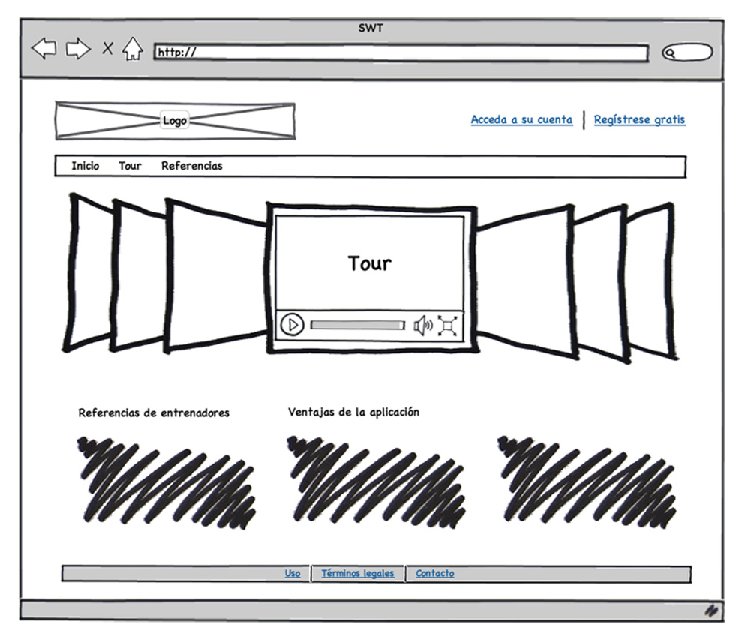
\includegraphics[width=8cm]{./eps/p_interfaz/1_Inicio.eps}
  	  \caption{Inicio en la interfaz pública}
  	  \label{fig:interfaz_publica_inicio}
  	\end{figure}

  	% subsection introducción (end)

  	\subsection{Interfaz pública} % (fold)
  		\label{sub:interfaz_publica}

  		La figura \ref{fig:interfaz_publica_inicio} muestra la estructura de la página web que actúa como interfaz pública. La parte superior está compuesta por el logo, enlace a registro/acceso a la aplicación y un menú para acceder al resto de páginas públicas a los entrenadores que aún no estén registrados en el sistema.

  		El resto de interfaces públicas que la conforman son: {\it tour} con las características y ventajas del sistema (figura \ref{fig:interfaz_publica_tour}); {\it referencias} de los entrenadores que participan en la elaboración del proyecto; página de {\it contacto} (figura \ref{fig:interfaz_publica_contacto}) con los administradores; {\it términos legales y de uso}. 

  		\begin{figure}[H]
  		  \centering
  		    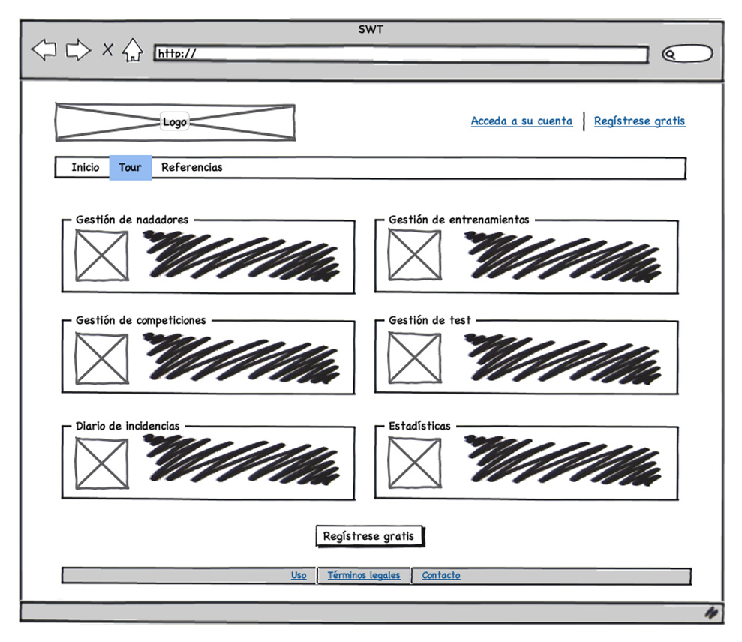
\includegraphics[width=8cm]{./eps/p_interfaz/2_Tour.eps}
  		  \caption{Tour en la interfaz pública}
  		  \label{fig:interfaz_publica_tour}
  		\end{figure}

  		\begin{figure}[H]
  		  \centering
  		    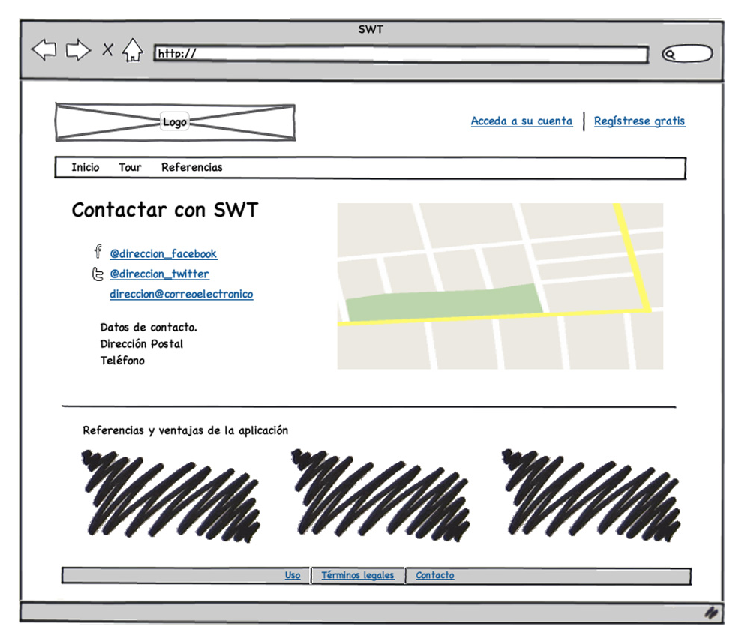
\includegraphics[width=8cm]{./eps/p_interfaz/3_Contacto.eps}
  		  \caption{Contacto en la interfaz pública}
  		  \label{fig:interfaz_publica_contacto}
  		\end{figure}

  	% subsection interfaz_pública (end)

  	\subsection{Registro y acceso} % (fold)
  		\label{sub:registro_y_acceso}

  		Las interfaces para el registro (figura \ref{fig:interfaz_registro}) y acceso (figura \ref{fig:interfaz_acceso}) de un entrenador al sistema son muy similares. Su estructura es algo diferente al resto de páginas de la aplicación, eliminando elementos que puedan interferir en el objetivo último ---registrarse o acceder. Hay que destacar que para el acceso, el identificador de usuario viene proporcionado por el correo electrónico insertado en la fase de registro.

  		\begin{figure}[H]
  		  \centering
  		    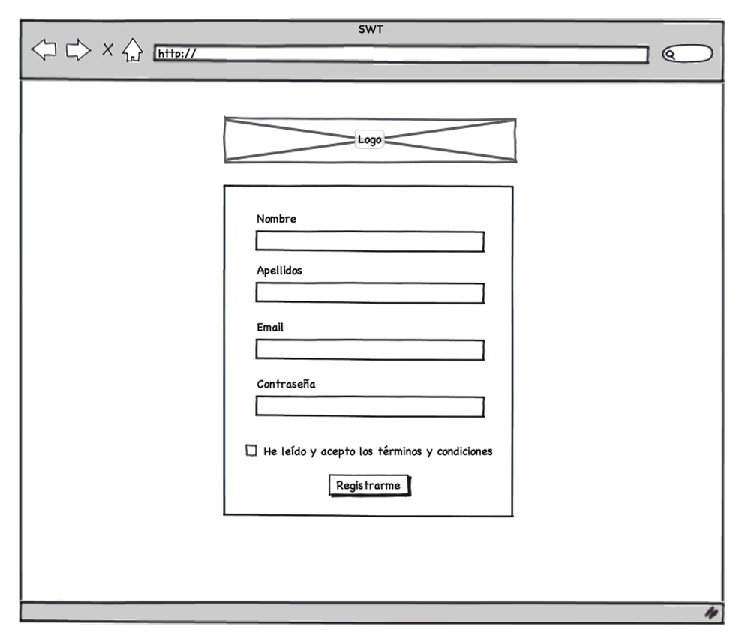
\includegraphics[width=8cm]{./eps/p_interfaz/4_Registro.eps}
  		  \caption{Interfaz para el registro de un entrenador}
  		  \label{fig:interfaz_registro}
  		\end{figure}

  		\begin{figure}[H]
  		  \centering
  		    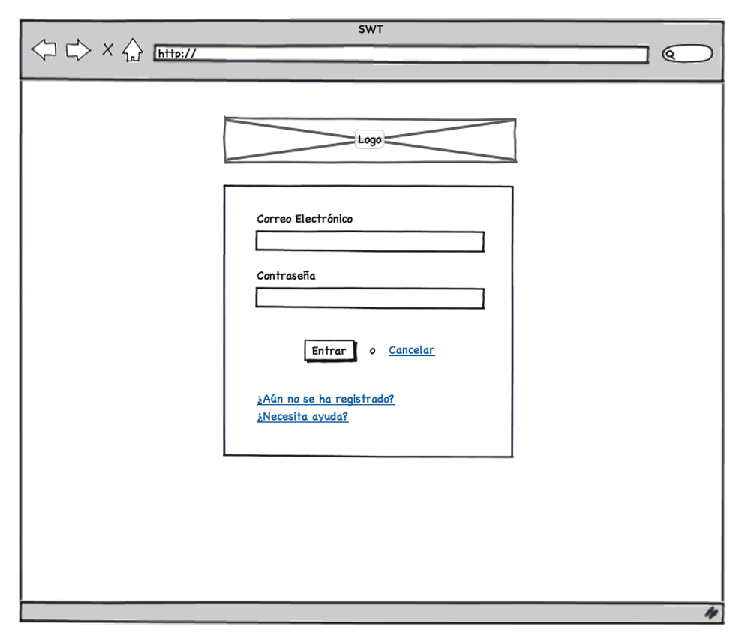
\includegraphics[width=8cm]{./eps/p_interfaz/5_Acceder.eps}
  		  \caption{Interfaz para el acceso de un entrenador}
  		  \label{fig:interfaz_acceso}
  		\end{figure}
  	% subsection registro_y_acceso (end)

  	\subsection{Dashboard} % (fold)
  		\label{sub:interfaz_dashboard}

  	Cuando el entrenador se registra en la aplicación, la primera página a la que accede es la de {\it dashboard} o resumen (figura \ref{fig:interfaz_dashboard}). En ella, lo primero que aparece es un recordatorio de los pasos que tiene que hacer para empezar a sacar provecho de la aplicación. A diferencia de las páginas vistas hasta el momento, ésta incluye en su estructura una barra lateral con los accesos que más frecuentemente se usan.

  		\begin{figure}[H]
  		  \centering
  		    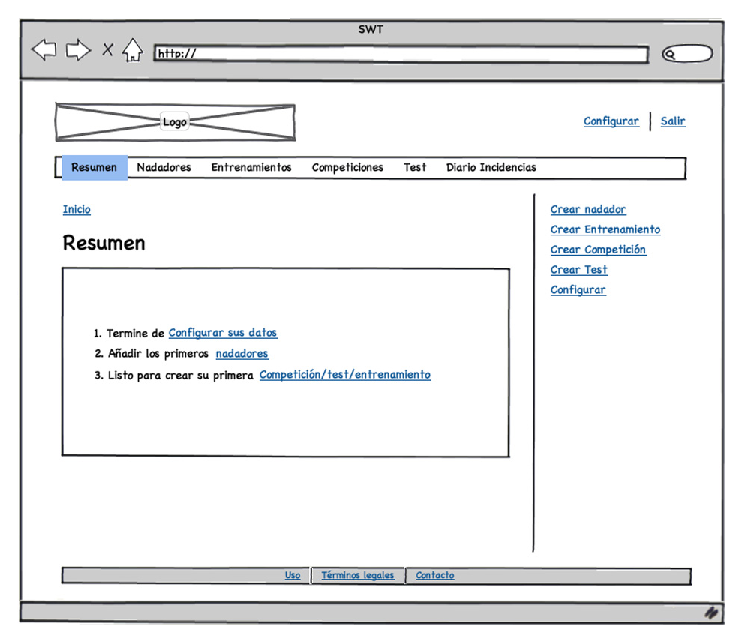
\includegraphics[width=8cm]{./eps/p_interfaz/6_Dashboard.eps}
  		  \caption{Interfaz para el dashboard de un entrenador}
  		  \label{fig:interfaz_dashboard}
  		\end{figure}

  	% subsection dashboard (end)

  	\subsection{Configuración del perfil} % (fold)
  		\label{sub:configuracion_del_perfil}

  	Cada entrenador registrado tiene un perfil asociado, donde se guarda información del tipo personal (figura \ref{fig:interfaz_conf_personal}), de contacto (figura \ref{fig:interfaz_conf_contacto}) y los parámetros relacionados con el índice de Mujika (figura \ref{fig:interfaz_conf_mujika}). La información está estructurada en pestañas para una mayor facilidad de navegación.

  		\begin{figure}[H]
  		  \centering
  		    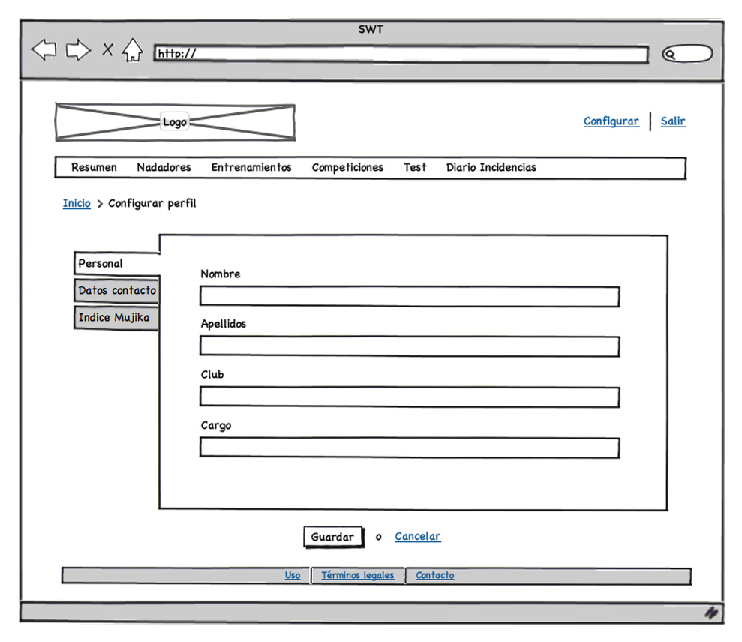
\includegraphics[width=8cm]{./eps/p_interfaz/7_Conf_personal.eps}
  		  \caption{Interfaz para la configuración de la información personal en el perfil}
  		  \label{fig:interfaz_conf_personal}
  		\end{figure}

  		\begin{figure}[H]
  		  \centering
  		    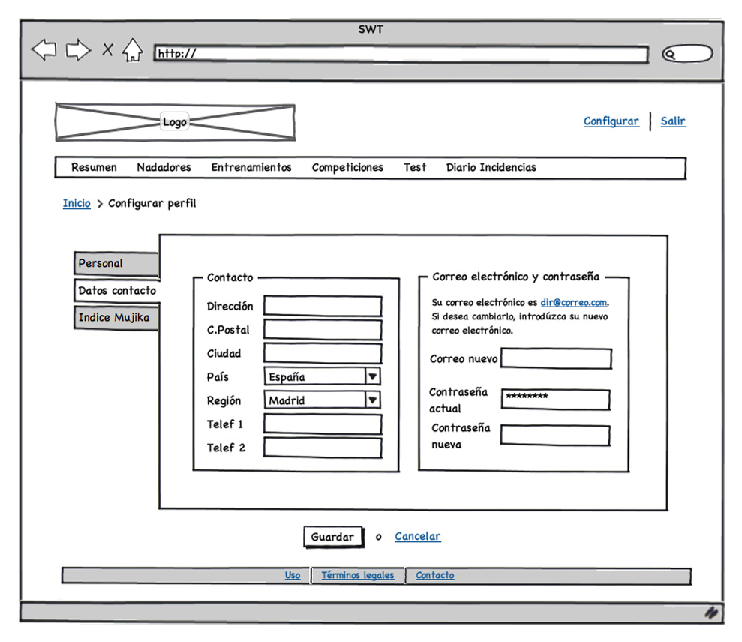
\includegraphics[width=8cm]{./eps/p_interfaz/8_Conf_contacto.eps}
  		  \caption{Interfaz para la configuración de la información de contacto en el perfil}
  		  \label{fig:interfaz_conf_contacto}
  		\end{figure}

  		\begin{figure}[H]
  		  \centering
  		    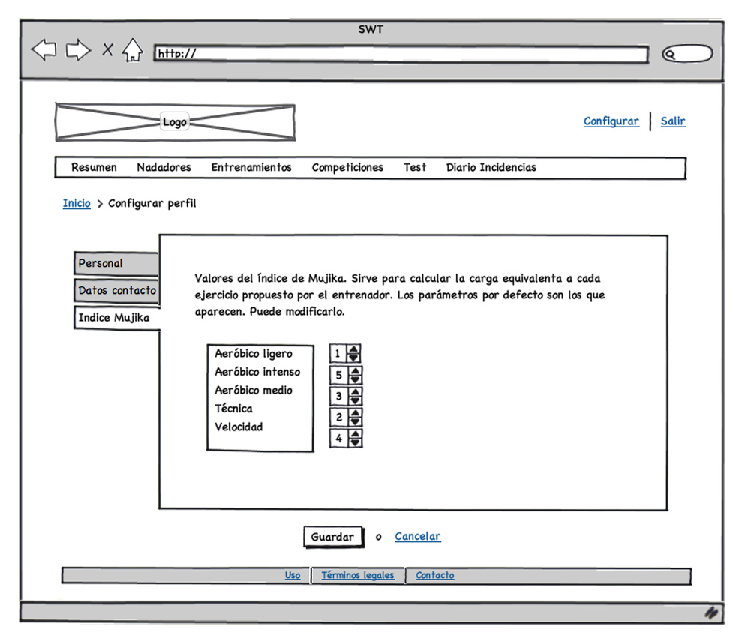
\includegraphics[width=8cm]{./eps/p_interfaz/9_Conf_mujika.eps}
  		  \caption{Interfaz para la configuración del índice de Mujika en el perfil}
  		  \label{fig:interfaz_conf_mujika}
  		\end{figure}

  	% subsection configuración_del_perfil (end)

  	\subsection{Gestión de nadadores} % (fold)
  		\label{sub:gestion_de_nadadores}

  	Uno de los módulos fundamentales en la aplicación es el de gestión de nadadores. Es, en gran medida, la base para las competiciones y los test, puesto que los resultados que se insertan en ellos dependen de los nadadores que un entrenador maneja. 

  	La estructura de la interfaz es común al resto de módulos y está compuesta de:

  	\begin{itemize}
  		\item {{\bf Tabla}. Muestra los registros insertados por un entrenador pertenecientes al módulo en que se encuentre. En este caso, como se está en la sección de nadadores, aparece el conjunto de nadadores que el entrenador ha dado de alta en el sistema.}
  		\item {{\bf Buscador}. Campo de búsqueda que localiza registros por diferentes parámetros.}
  		\item {{\bf Resumen}. Muestra información relevante al módulo en que se encuentre. Lo normal es que aparezca el número de registros insertados en cada módulo.}
  		\item {{\bf Barra lateral}. Desde ella se accede a cada una de las opciones del módulo que se esté gestionando.}
  	\end{itemize}

  	A continuación se muestran las interfaces de {\it ver listado de nadadores} (figura \ref{fig:interfaz_nadadores}), {\it añadir nadador} (figura \ref{fig:interfaz_nadadores_new}), {\it ver nadador} (figura \ref{fig:interfaz_nadadores_show}) y {\it modificar nadador} (figura \ref{fig:interfaz_nadadores_modif}). La primera de ellas muestra todos los nadadores insertados en la aplicación por un entrenador registrado; la segunda refleja el proceso para añadir un nuevo nadador; y la tercera como se modificaría. Es destacable que la información relacionada con las competiciones y test que aparece en {\it ver nadador}, no pueden ser modificadas desde este módulo, sino desde los que gestionan las competiciones y test.

  	\begin{figure}[H]
  	  \centering
  	    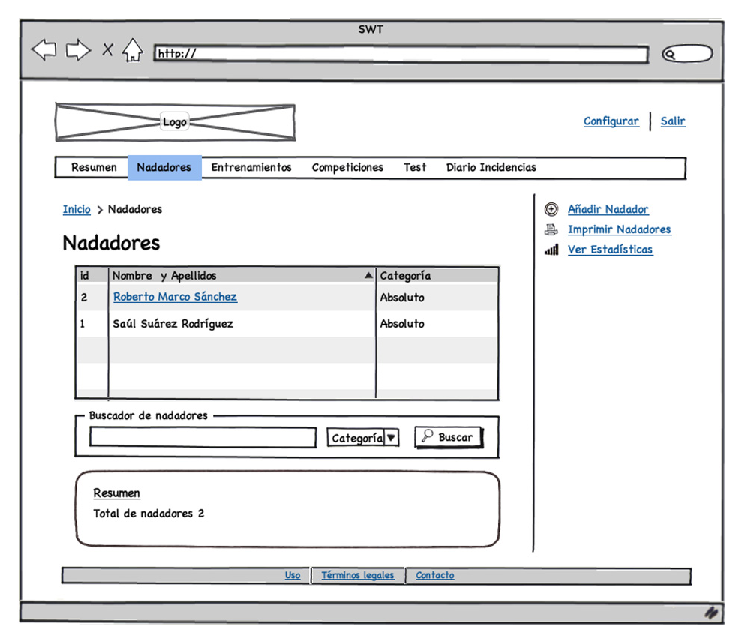
\includegraphics[width=8cm]{./eps/p_interfaz/10_Nadadores.eps}
  	  \caption{Interfaz para ver listado de nadadores}
  	  \label{fig:interfaz_nadadores}
  	\end{figure}

  	\begin{figure}[H]
  	  \centering
  	    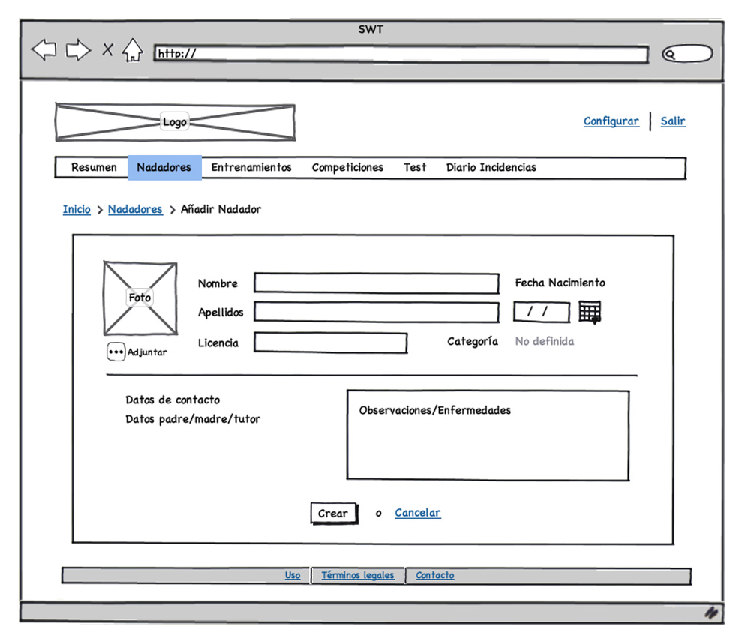
\includegraphics[width=8cm]{./eps/p_interfaz/11_Nadadores_new.eps}
  	  \caption{Interfaz para añadir nadador}
  	  \label{fig:interfaz_nadadores_new}
  	\end{figure}

  	\begin{figure}[H]
  	  \centering
  	    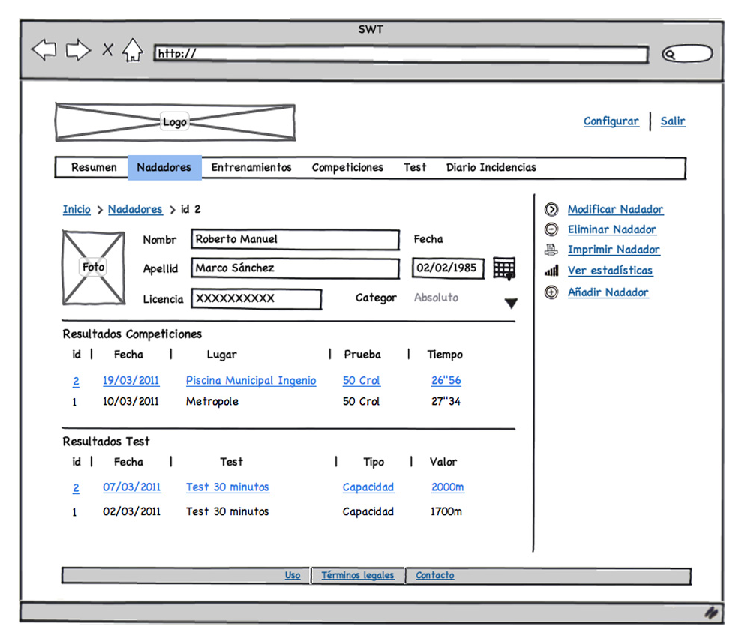
\includegraphics[width=8cm]{./eps/p_interfaz/12_Nadadores_show.eps}
  	  \caption{Interfaz para ver nadador}
  	  \label{fig:interfaz_nadadores_show}
  	\end{figure}

  	\begin{figure}[H]
  	  \centering
  	    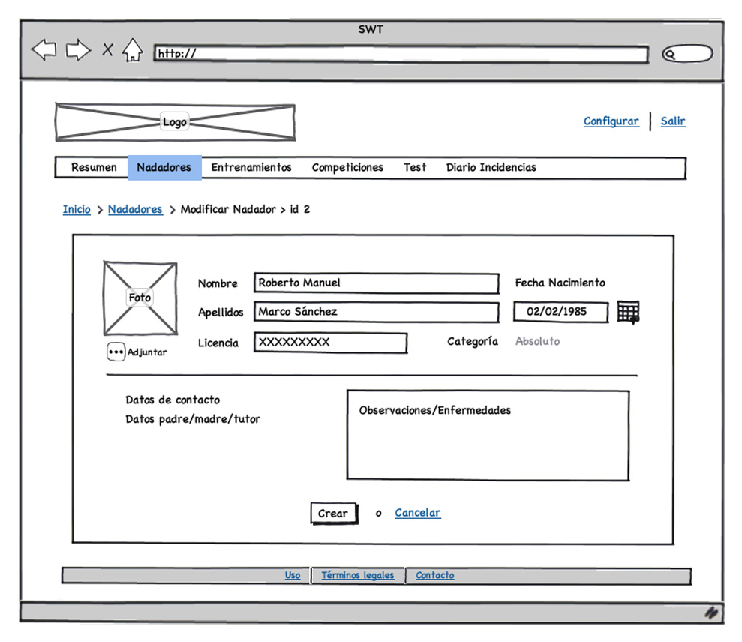
\includegraphics[width=8cm]{./eps/p_interfaz/13_Nadadores_modif.eps}
  	  \caption{Interfaz para modificar nadador}
  	  \label{fig:interfaz_nadadores_modif}
  	\end{figure}
  	% subsection gestión_de_nadadores (end)

  	\subsection{Gestión de Competiciones} % (fold)
  		\label{sub:gestion_de_competiciones}

  	La figura \ref{fig:interfaz_competiciones} muestra la interfaz para ver las competiciones añadidas por un entrenador registrado. Su estructura, como se especificó anteriormente, es similar a la del resto de módulos. La particularidad que tiene es que aparece un calendario de la temporada. A medida que se {\it añadan competiciones} (figura \ref{fig:interfaz_competiciones_new}) irán apareciendo ahí. 

  		\begin{figure}[H]
  		  \centering
  		    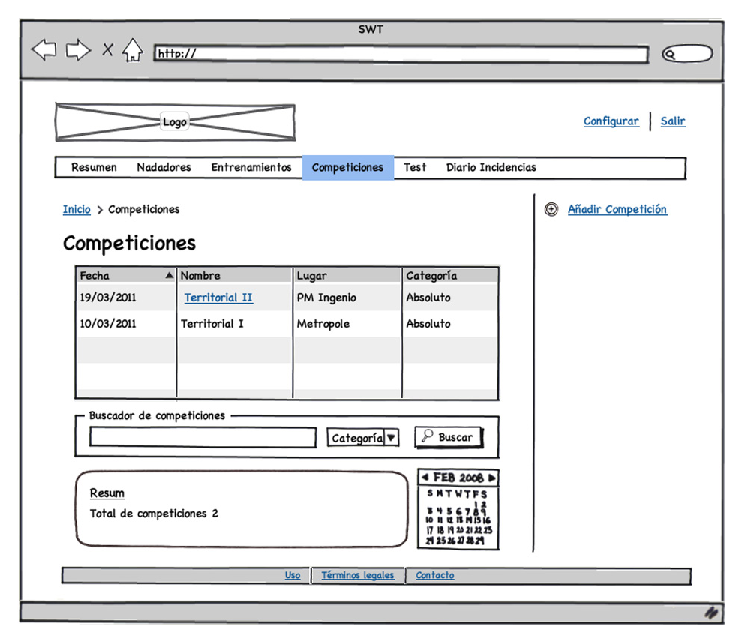
\includegraphics[width=8cm]{./eps/p_interfaz/14_Competiciones.eps}
  		  \caption{Interfaz para ver listado de competiciones}
  		  \label{fig:interfaz_competiciones}
  		\end{figure}

  		\begin{figure}[H]
  		  \centering
  		    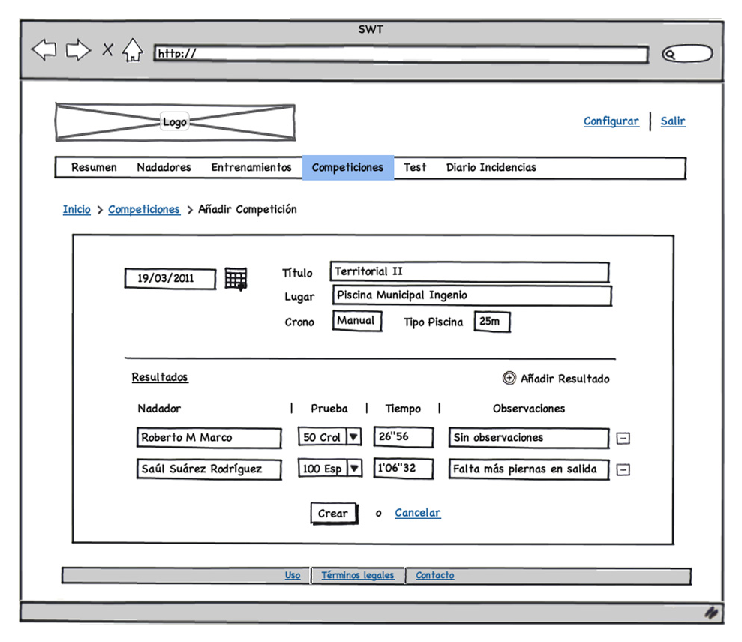
\includegraphics[width=8cm]{./eps/p_interfaz/15_Competiciones_new.eps}
  		  \caption{Interfaz para añadir competición}
  		  \label{fig:interfaz_competiciones_new}
  		\end{figure}

  Cuando un entrenador hace clic sobre el nombre de la competición en la tabla, se accede a {\it ver una competición} (figura \ref{fig:interfaz_competiciones_show}). Cuando se modifica una competición (figura \ref{fig:interfaz_competiciones_modif}), se da la posibilidad de modificar cada uno de los resultados añadidos a la misma. Esta información es la que aparecerá modificada en la ficha de cada nadador.

  		\begin{figure}[H]
  		  \centering
  		    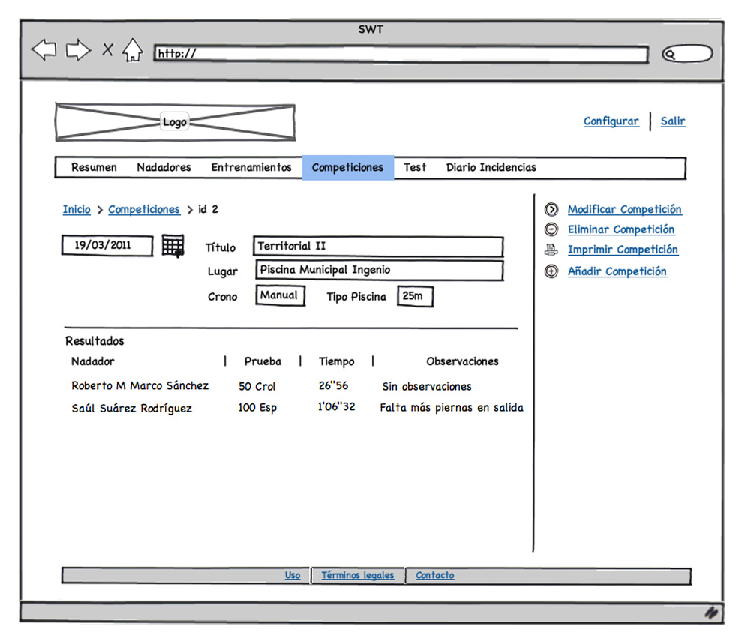
\includegraphics[width=8cm]{./eps/p_interfaz/16_Competiciones_show.eps}
  		  \caption{Interfaz para ver competición}
  		  \label{fig:interfaz_competiciones_show}
  		\end{figure}

  		\begin{figure}[H]
  		  \centering
  		    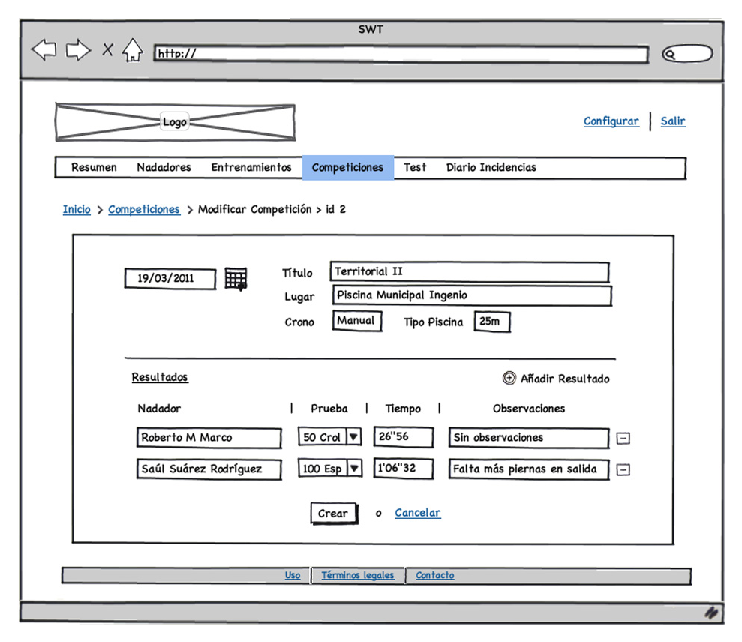
\includegraphics[width=8cm]{./eps/p_interfaz/17_Competiciones_modif.eps}
  		  \caption{Interfaz para modificar competición}
  		  \label{fig:interfaz_competiciones_modif}
  		\end{figure}
  	% subsection gestión_de_competiciones (end)

  	\subsection{Gestión de entrenamientos} % (fold)
  		\label{sub:gestion_de_entrenamientos}

  		\begin{figure}[H]
  		  \centering
  		    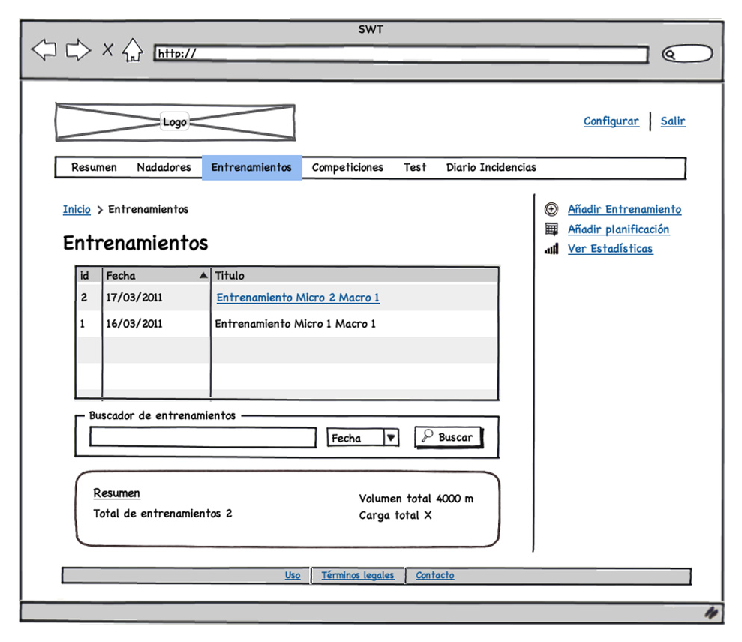
\includegraphics[width=8cm]{./eps/p_interfaz/18_Entrenamientos.eps}
  		  \caption{Interfaz para ver listado de entrenamientos}
  		  \label{fig:interfaz_entrenamientos}
  		\end{figure}

  	La {\it lista de entrenamientos} (figura \ref{fig:interfaz_entrenamientos}) refleja cada una de las sesiones que inserta el entrenador a lo largo de una temporada. En el resumen se muestran la cantidad de sesiones, el volumen y la carga realizadas en total. Al hacer clic sobre el nombre del entrenamiento, se accede a {\it ver entrenamiento} (figura \ref{fig:interfaz_entrenamientos_show}), que incluye cada uno de los ejercicios añadidos al mismo. Como cada ejercicio tiene asociado un volumen y una carga, se muestra el total de esa sesión. Esto ayuda al entrenador a la hora de hacer los entrenamientos, puesto que conoce el estado a medida que los va desarrollando.\\
  	\newline
  	{\it Añadir} (figura \ref{fig:interfaz_entrenamientos_new}) y {\it modificar entrenamiento} son iguales, con la salvedad de que el segundo permite cambiar los datos de los formularios que se agregan en el primero.

  		\begin{figure}[H]
  		  \centering
  		    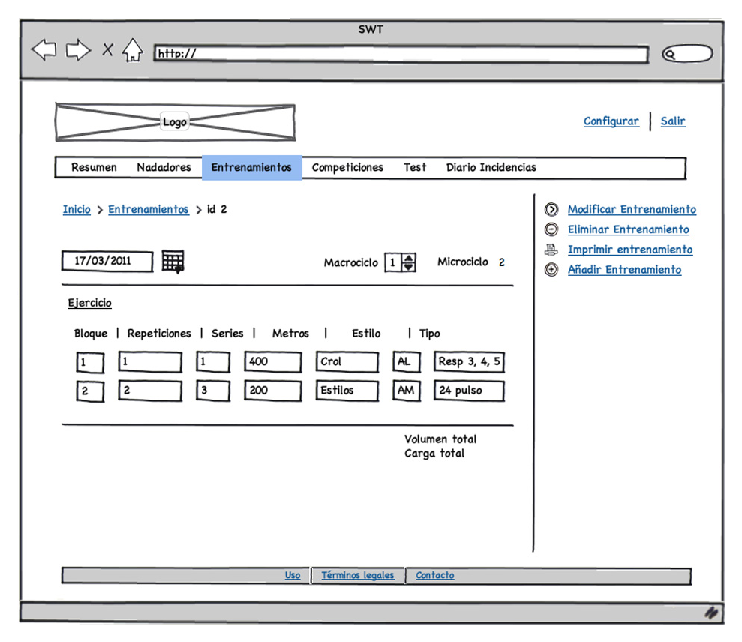
\includegraphics[width=8cm]{./eps/p_interfaz/20_Entrenamientos_show.eps}
  		  \caption{Interfaz para ver entrenamiento}
  		  \label{fig:interfaz_competiciones_show}
  		\end{figure}

  		\begin{figure}[H]
  		  \centering
  		    \includegraphics[width=8cm]{./eps/p_interfaz/19_Entrenamientos_new.eps}
  		  \caption{Interfaz para añadir entrenamiento}
  		  \label{fig:interfaz_entrenamientos_new}
  		\end{figure}

  	% subsection gestión_de_entrenamientos (end)

  	\subsection{Gestión de test} % (fold)
  		\label{sub:gestion_de_test}

  	Al igual que para las competiciones, la gestión de test (figura \ref{fig:interfaz_test}) se realiza de la misma forma. La diferencia fundamental está en la información que aparece en la tabla de test insertados por el entrenador en la aplicación. Como para las competiciones, cada uno de los resultados asociados a cada test, aparecen en la ficha de cada nadador.

  		\begin{figure}[H]
  		  \centering
  		    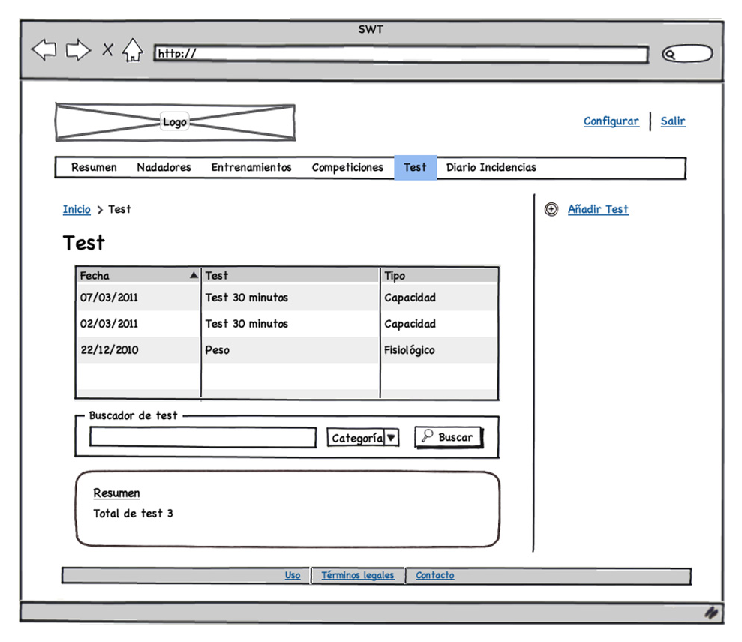
\includegraphics[width=8cm]{./eps/p_interfaz/26_Test.eps}
  		  \caption{Interfaz para ver listado de test}
  		  \label{fig:interfaz_test}
  		\end{figure}
  	% subsection gestión_de_test (end)

  	\subsection{Gestión diario de incidencias} % (fold)
  		\label{sub:interfaz_gestion_diario_de_incidencias}

  	La interfaz para el diario de incidencias del entrenador difiere del resto en que, cada incidencia, tiene asociada una o varias etiquetas. Por ello, en el resumen que aparece en la interfaz de {\it ver diario de incidencias} (figura \ref{fig:interfaz_incidencias}), se muestran los valores más usados por los entrenadores. Esto ayudará a localizar rápidamente cada tipo de incidencia. Como en casos anteriores, a continuación se muestra {\it ver incidencia} (figura \ref{fig:interfaz_incidencias_show}), {\it añadir incidencia} (figura \ref{fig:interfaz_incidencias_new}) y {\it modificar incidencia} (figura \ref{fig:interfaz_incidencias_modif}).

  		\begin{figure}[H]
  		  \centering
  		    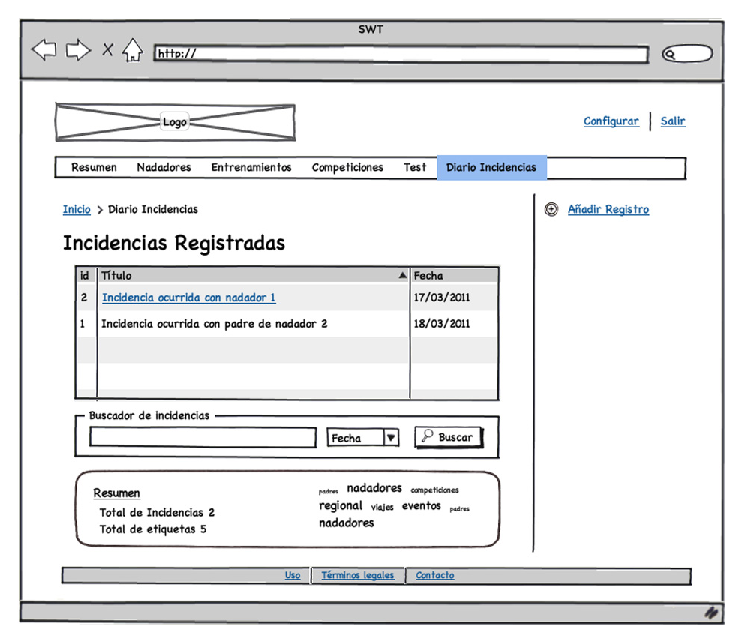
\includegraphics[width=8cm]{./eps/p_interfaz/22_Diario.eps}
  		  \caption{Interfaz para ver diario de incidencias}
  		  \label{fig:interfaz_incidencias}
  		\end{figure}

  		\begin{figure}[H]
  		  \centering
  		    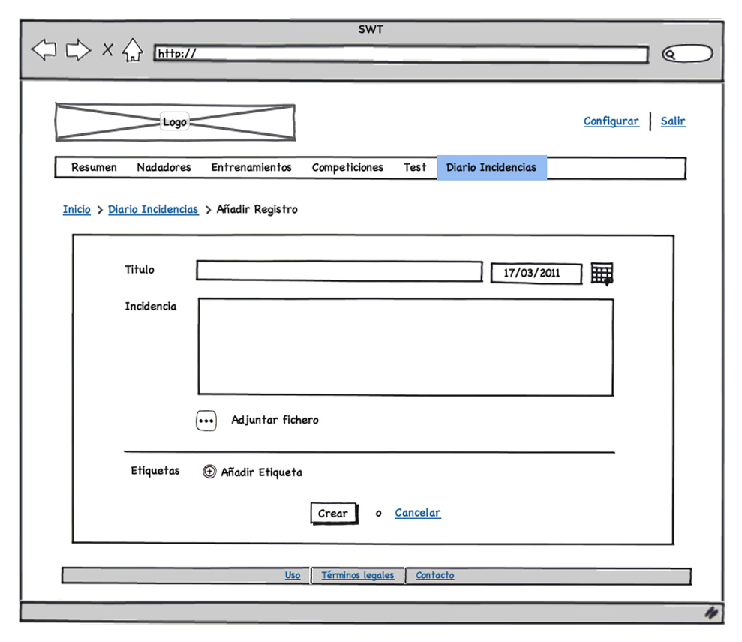
\includegraphics[width=8cm]{./eps/p_interfaz/23_Diario_new.eps}
  		  \caption{Interfaz para añadir incidencia}
  		  \label{fig:interfaz_incidencias_new}
  		\end{figure}

  		\begin{figure}[H]
  		  \centering
  		    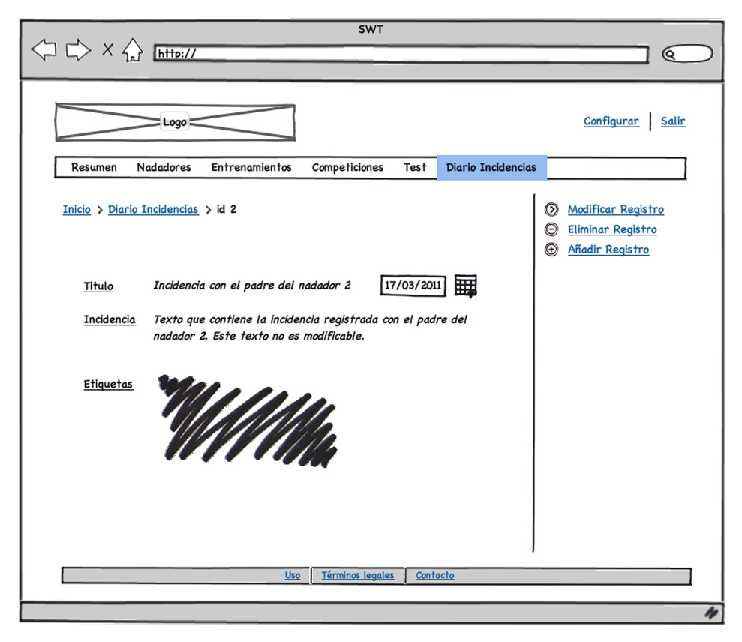
\includegraphics[width=8cm]{./eps/p_interfaz/24_Diario_show.eps}
  		  \caption{Interfaz para ver incidencia}
  		  \label{fig:interfaz_incidencias_show}
  		\end{figure}

  		\begin{figure}[H]
  		  \centering
  		    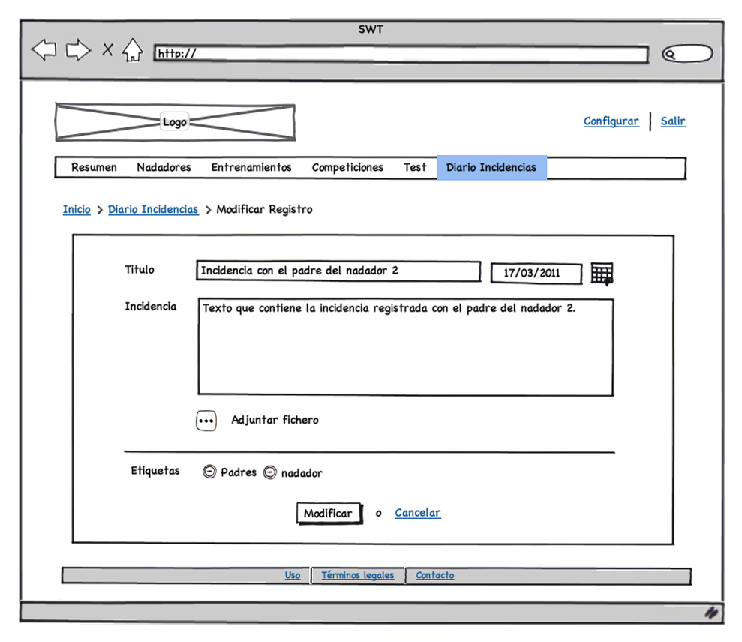
\includegraphics[width=8cm]{./eps/p_interfaz/25_Diario_modif.eps}
  		  \caption{Interfaz para modificar incidencia}
  		  \label{fig:interfaz_incidencias_modif}
  		\end{figure}
  	% subsection interfaz_gestión_diario_de_incidencias (end)
  % section diseño_de_interfaz_de_usuario (end)
  
	% ----------------------------------
	% Sec Diagramas clases
	% ----------------------------------
	\section{Diagramas de clases} % (fold)
		\label{sec:diagramas_de_clases}
		
		Una clase de diseño y sus objetos, y de ese modo también los subsistemas que contienen las clases de diseño, a menudo participan en varias realizaciones de casos de uso. También puede darse el caso de algunas operaciones, atributos y asociaciones sobre una clase específica que son relevantes para sólo una realización de caso de uso. Esto es importante para coordinar todos los requisitos que diferentes realizaciones de casos de uso imponen a una clase, a sus objetos y a los subsistemas que que contiene. Para manejar todo esto, se utilizan los diagramas de clases conectados a una realización de caso de uso, mostrando sus clases participantes, subsistemas y sus relaciones. 
		
		% ----------------------------------
		% Sub Patrón MVC
		% ----------------------------------
		\subsection{Patrón MVC} % (fold)
			\label{sub:patron_mvc}
			
			MVC es un patrón de diseño que considera dividir una aplicación en tres módulos claramente identificables y con funcionalidad bien definida: {\it el modelo, las vistas y el controlador}.
			
			\begin{itemize}
				\item {\bf El modelo} es un conjunto de clases que representan la información del mundo real que el sistema debe procesar, sin tomar en cuenta ni la forma en la que esa información va a ser mostrada ni los mecanismos que hacen que esos datos estén dentro del modelo, es decir, sin tener relación con ninguna otra entidad dentro de la aplicación. 
				\item {\bf Las vistas} son el conjunto de clases que se encargan de mostrar al usuario la información contenida en el modelo. Una vista está asociada a un modelo, pudiendo existir varias vistas asociadas al mismo modelo. Una vista obtiene del modelo solamente la información que necesita para desplegar y se actualiza cada vez que el modelo del dominio cambia por medio de notificaciones generadas por el modelo de la aplicación.
				\item {\bf El controlador} es un objeto que se encarga de dirigir el flujo del control de la aplicación debido a mensajes externos, como datos introducidos por el usuario u opciones del menú seleccionadas por él. A partir de estos mensajes, el controlador se encarga de modificar el modelo o de abrir y cerrar vistas. El controlador tiene acceso al modelo y a las vistas, pero las vistas y el modelo no conocen de la existencia del controlador.
			\end{itemize}			
			
			\begin{figure}[H]
			  \centering
			    \includegraphics[width=12cm]{./eps/di_diagclases/mvc.eps}
			  \caption{Disposición en el patrón MVC}
			  \label{fig:patron_MVC}
			\end{figure}
			
			Aunque se pueden encontrar diferentes implementaciones de MVC, el flujo que sigue el control generalmente es el siguiente:
			
			\begin{itemize}
				\item El usuario interactúa con la interfaz de usuario de alguna forma.
				\item El controlador recibe (por parte de los objetos de la interfaz-vista) la notificación de la acción solicitada por el usuario. El controlador gestiona el evento que llega. 
				\item El controlador accede al modelo, actualizándolo, posiblemente modificándolo de forma adecuada a la acción solicitada por el usuario. Los controladores complejos están a menudo estructurados usando un patrón de comando que encapsula las acciones y simplifica su extensión.
				\item El controlador delega a los objetos de la vista la tarea de desplegar la interfaz de usuario. La vista obtiene sus datos del modelo para generar la interfaz apropiada para el usuario donde se reflejan los cambios en el modelo. El modelo no debe tener conocimiento directo sobre la vista. El controlador no pasa objetos de dominio (el modelo) a la vista aunque puede dar la orden a la vista para que se actualice. 
				\item La interfaz de usuario espera nuevas interacciones del usuario, comenzando el ciclo nuevamente. 
			\end{itemize}
			
			La disposición de los paquetes de la aplicación se organizarán según el patrón MVC ({\it véase} Figura \ref{fig:patron_MVC}). Por ello, los modelos, los controladores y las vistas se encontrarán aisladas entre sí.
			
			Para simplificar el diagrama de clases de la aplicación, en la figura \ref{fig:di_diag_clases} se muestran las clases con los estereotipos usados en el {\it framework} de desarrollo, agrupando únicamente las pertenecientes al modelo.
			
			\begin{figure}[H]
			  \centering
			    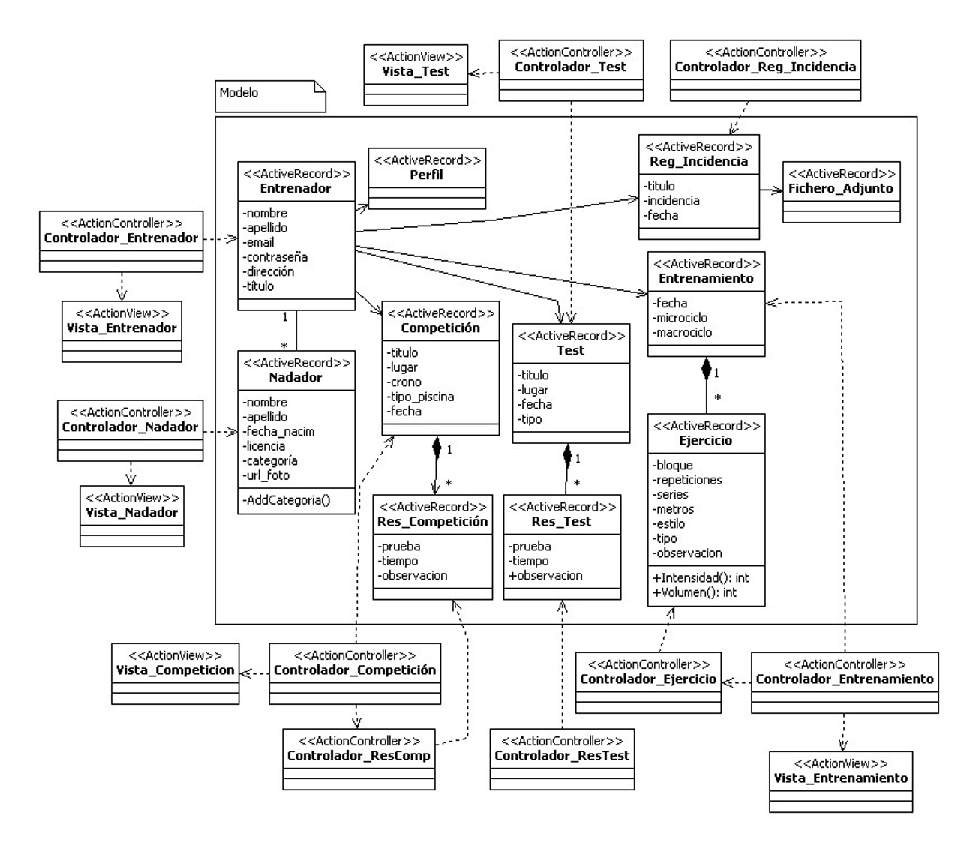
\includegraphics[width=16cm]{./eps/di_diagclases/di_diagclases.eps}
			  \caption{Diagrama de clases para el diseño}
			  \label{fig:di_diag_clases}
			\end{figure}
			
			Los controladores se relacionan directamente con las vistas y los modelos, habiendo tal y como se explicó anteriormente, una separación lógica entre vistas y modelos.
			
			El {\bf Modelo} es donde residen los datos y es el encargado de acceder a los mismos. Se comunica con el gestor de bases de datos para que se realice todo el almacenamiento de estos. En las aplicaciones basadas en {\it Ruby on Rails}, la definición del modelo es sumamente importante, puesto que el modelo de negocio se sustenta en él.

    	 \begin{figure}[H]
    		  \centering
    		    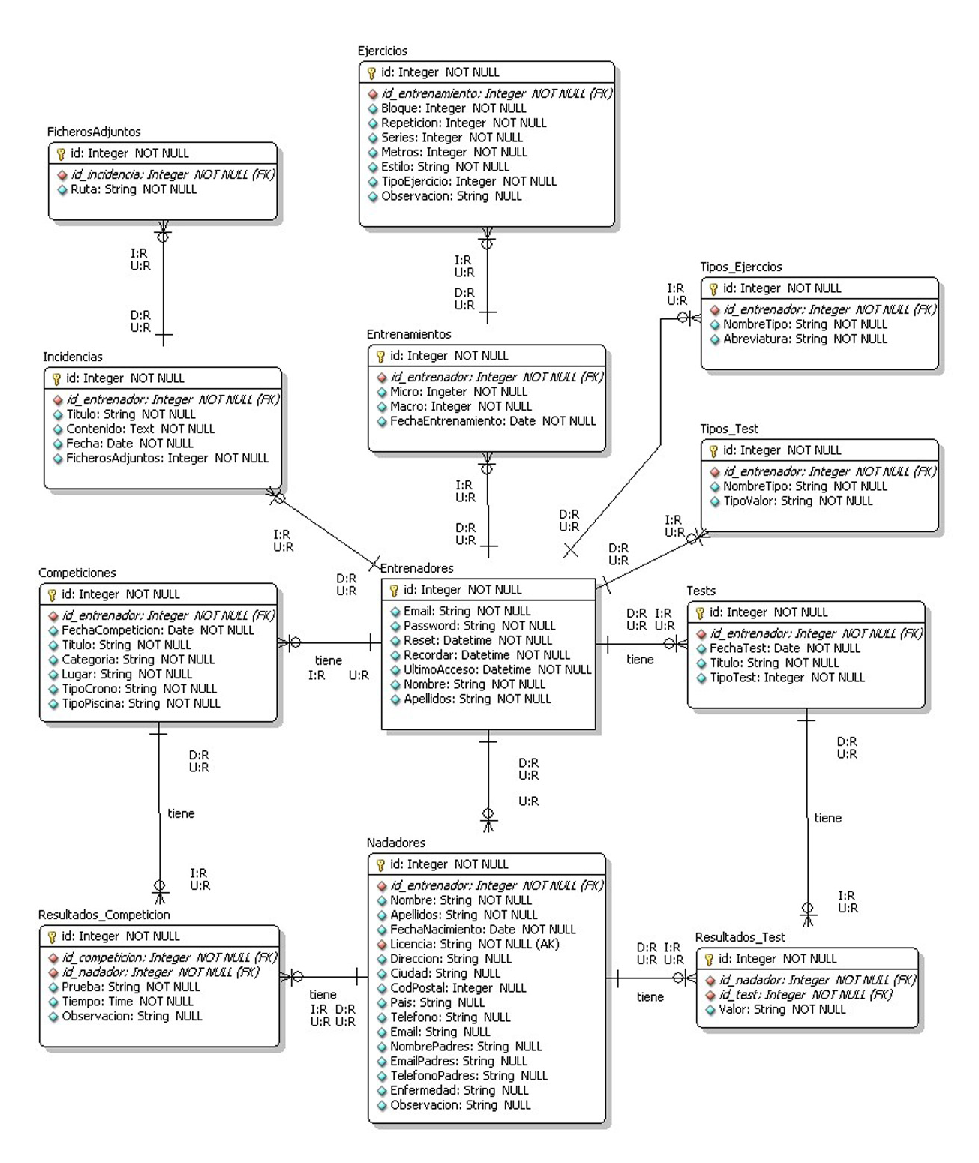
\includegraphics[width=13cm]{./eps/di_modelo_er/ModeloER.eps}
    		  \caption{Estructuración del modelo de bases de datos}
    		  \label{fig:di_diag_despliegue}
    		\end{figure}
			
		% subsection patrón_mvc (end)
		
	% section diagramas_de_clases (end)
	
	% ----------------------------------
	% Sec Diagramas de Secuencia
	% ----------------------------------
	\section{Diagramas de secuencia} % (fold)
		\label{sec:diagramas_de_secuencia}
	
		Cómo fue explicado en capítulos anteriores, los diagramas de interacción son diagramas que describen cómo grupos de objetos colaboran para conseguir algún fin. Estos diagramas muestran objetos, así como los mensajes que se pasan entre ellos dentro del caso de uso, es decir, capturan el comportamiento de los casos de uso.
		
		La secuencia de acciones en un caso de uso comienza cuando un actor invoca el caso de uso mediante el envío de algún tipo de mensaje al sistema. Si se considera el <<interior>> del sistema, se tiene algún objeto de diseño que recibe el mensaje del actor. Después el objeto de diseño llama a algún otro objeto, y de esa manera los objetos implicados interactúan para realizar y llevar a cabo un caso de uso. En el diseño, es preferible representar esto con diagramas de secuencia, ya que el centro de atención principal es el encontrar secuencias de interacciones detalladas y ordenadas en el tiempo.
		
		Hay dos tipos de diagrama de interacción, ambos basados en la misma información, pero cada uno enfatizando un aspecto particular: {\bf Diagramas de Secuencia} y Diagramas de Colaboración.
		
		Un diagrama de secuencia muestra una interacción ordenada según la secuencia temporal de eventos. En particular, muestra los objetos participantes en la interacción y los mensajes que intercambian ordenados según su secuencia en el tiempo. Es decir, muestra la interacción de un conjunto de objetos en una aplicación a través del tiempo y se modela para cada caso de uso.
		
		A continuación se detallarán dos diagramas de secuencia que hacen referencia a la cada uno de los módulos detallados en la fase de análisis (capítulo \ref{cha:analisis}).
		
		Se recuerda al lector que los paquetes principales son:
		\begin{itemize}
		  \item Gestión de nadadores
		  \item Gestión de competiciones
		  \item Gestión de test
		  \item Gestión del diario de incidencias
		\end{itemize}
		
		% ----------------------------------
		% Sub Diagrama secuencia añadir nadador
		% ----------------------------------
		\subsection{Diagrama secuencia añadir nadador} % (fold)
		\label{sub:diagrama_secuencia_anadir_nadador}
			
			En el diagrama de secuencia de la figura \ref{fig:di_sec_anadirnadador} se muestra el flujo de acciones correspondiente para poder crear un nuevo nadador en el sistema.
			
			La clase {\it Vista Nadador} engloba las vistas correspondientes a cada uno de los métodos del controlador de nadadores. Así, por ejemplo, al método {\it index} del controlador le corresponde una vista {\it index.html.erb}. Es fundamental conocer esto para entender que en las acciones 3 y 7 el controlador envía la acción de renderizar las vistas correspondientes a los métodos {\it new y show}, debido a que son los que se ejecutan dentro de la clase.
			
			La clase {\it nadador} correspondiente al modelo es la encargada de detectar si es posible la creación de un nuevo registro o no en la base de datos. En caso de no ser posible, notifica al controlador y éste muestra un mensaje de error en la vista. En caso de que todo vaya bien, se muestra el nuevo registro creado con la ficha del nadador.
			
			\begin{figure}[H]
			  \centering
			    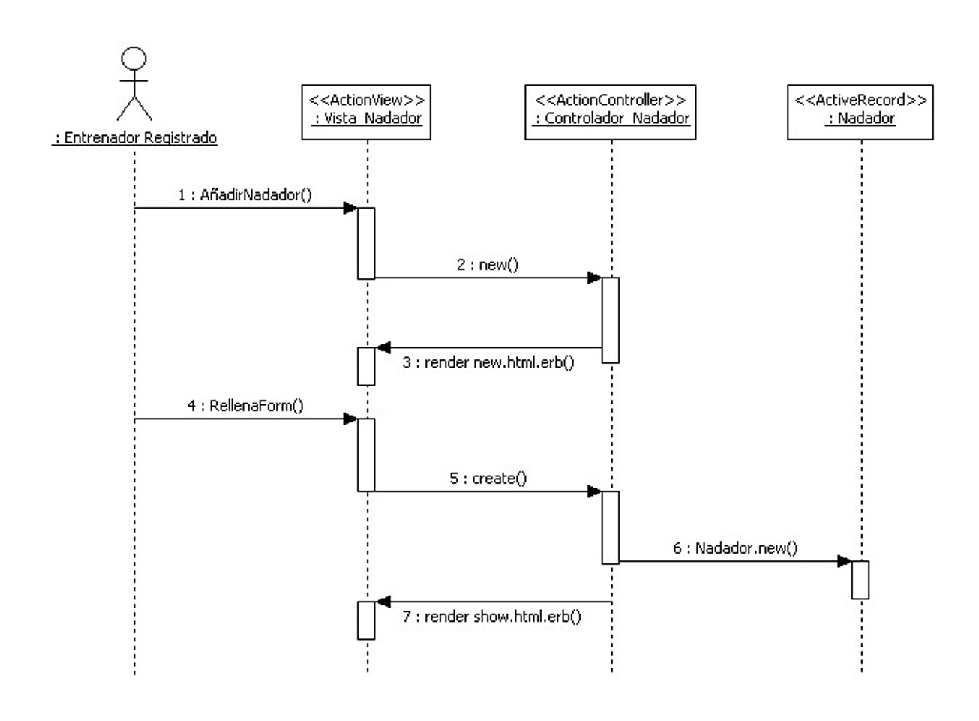
\includegraphics[width=15cm]{./eps/di_diagsecuencia/Nadador_Anadir.eps}
			  \caption{Diagrama de secuencia para añadir un nadador}
			  \label{fig:di_sec_anadirnadador}
			\end{figure}
			
		% subsection diagrama_secuencia_añadir_nadador (end) 
		
		% ----------------------------------
		% Sub Diagrama secuencia ver nadador
		% ----------------------------------
		\subsection{Diagrama secuencia ver nadador} % (fold)
		\label{sub:diagrama_secuencia_ver_nadador}
		
			En el diagrama de secuencia de la figura \ref{fig:di_sec_anadirnadador} se muestra el flujo de acciones correspondiente para poder ver un nadador perteneciente a un entrenador registrado.
			
			La secuencia comienza cuando el entrenador registrado solicita ver el listado de nadadores que ha añadido al sistema. Es requisito el ver el listado para poder posteriormente seleccionar un nadador concreto. Para ver todo el conjunto de nadadores, el controlador obtiene del modelo todos los nadadores y los muestra al renderizar {\it index.html.erb}. 
			
			El siguiente paso es el {\it seleccionar un nadador} concreto. Se hace una llamada al método {\it show}, el cuál pedirá al modelo el nadador concreto seleccionado. El modelo devuelve los datos del nadador y el controlador renderizará la ficha del mismo.
			
			Requisitos que se tendrán que contemplar en la fase de implementación:
			
			\begin{itemize}
			 \item No se puede acceder a un nadador perteneciente a otro nadador.
			 \item En caso de no poderse acceder, se mostrará mensaje de error.
			\end{itemize}
			
			\begin{figure}[H]
			  \centering
			    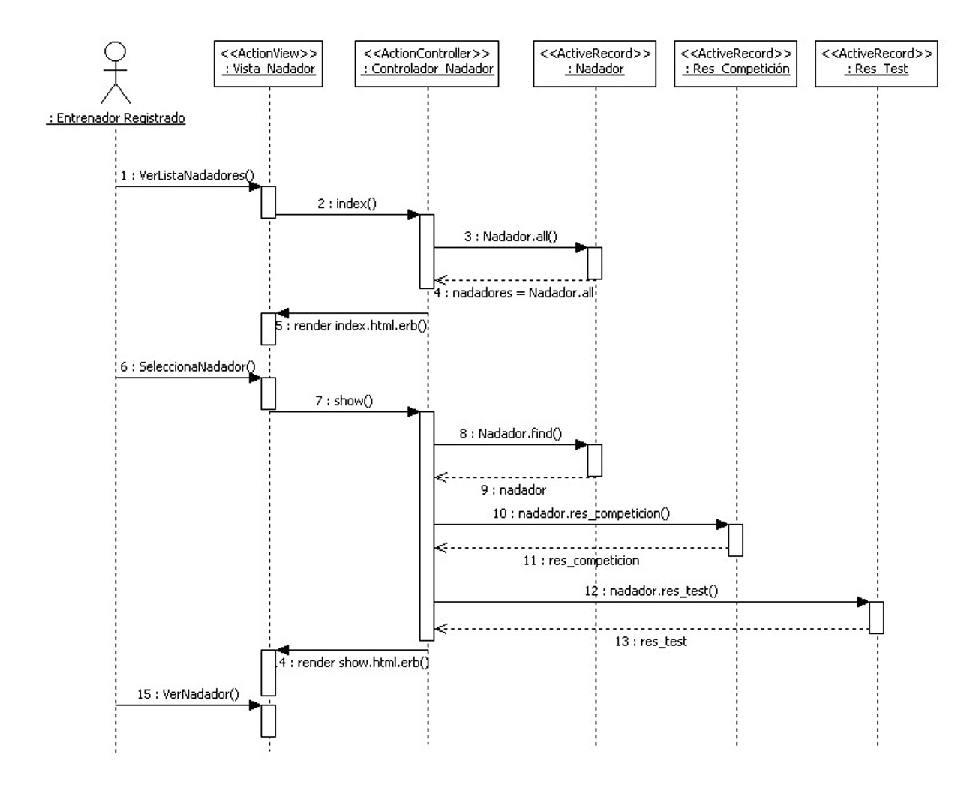
\includegraphics[width=15cm]{./eps/di_diagsecuencia/Nadador_Ver.eps}
			  \caption{Diagrama de secuencia para ver un nadador}
			  \label{fig:di_sec_vernadador}
			\end{figure}
		
		% subsection diagrama_secuencia_ver_lista_de_nadadores (end)
		
		% ----------------------------------
		% Sub Diagrama secuencia eliminar nadador
		% ----------------------------------
		\subsection{Diagrama secuencia eliminar nadador} % (fold)
		  \label{sub:diagrama_secuencia_eliminar_nadador}
		
		  En el diagrama de secuencia de la figura \ref{fig:di_sec_eliminarnadador} se muestra el flujo de acciones correspondiente para poder eliminar un nadador del sistema.
		  
		  Primeramente el entrenador ve la lista de nadadores insertados en el sistema a través de la clase {\it Vista Nadador}. Esto es requisito para poder seleccionar el candidato a eliminar. Una vez elegido, se lanzará el método {\it destroy} desde el controlador, el cuál indicará al modelo que se destruya el registro almacenado en el modelo. Así mismo, se realizará el correspondiente borrado en cascada de la información correspondiente a los resultados almacenados sobre competiciones y test pertenecientes al nadador.
		  
		  \begin{figure}[H]
			  \centering
			    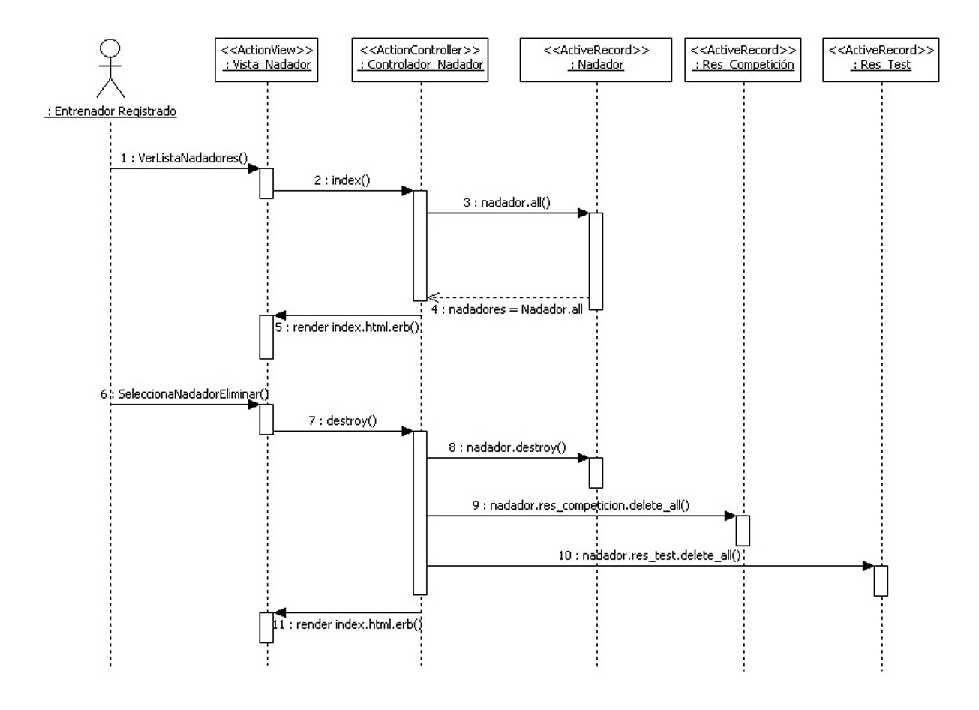
\includegraphics[width=15cm]{./eps/di_diagsecuencia/Nadador_Eliminar.eps}
			  \caption{Diagrama de secuencia para eliminar un nadador}
			  \label{fig:di_sec_eliminarnadador}
			\end{figure}
		% subsection diagrama_secuencia_eliminar_nadador (end)
		
		% ----------------------------------
		% Sub Diagrama secuencia modificar nadador
		% ----------------------------------
		\subsection{Diagrama secuencia modificar nadador} % (fold)
		  \label{sub:diagrama_secuencia_modificar_nadador}
		  
		  En el diagrama de secuencia de la figura \ref{fig:di_sec_modificarnadador} se muestra el flujo de acciones correspondiente para poder modificar un nadador perteneciente a un entrenador determinado del sistema.
		  
		  El flujo de sucesos comienza con la selección por parte del entrenador de la opción {\it Ver lista de nadadores}. Una vez mostrados, se selecciona el candidato a modificar. Es el propio controlador quien llama primeramente al método {\it edit}, donde se muestra un formulario con los datos del nadador almacenados en el modelo. Posteriormente, el {\it Controlador Nadador} renderizará la vista para poder editar los datos.
		
		  Requisito que se tendrá que contemplar en la fase de implementación:
			
			\begin{itemize}
			 \item Únicamente se podrán modificar los datos del modelo de nadador en la {\it Vista Entrenamiento}. Los resultados en competiciones y test no se podrán cambiar desde esta vista.
			\end{itemize}
			
		  \begin{figure}[H]
			  \centering
			    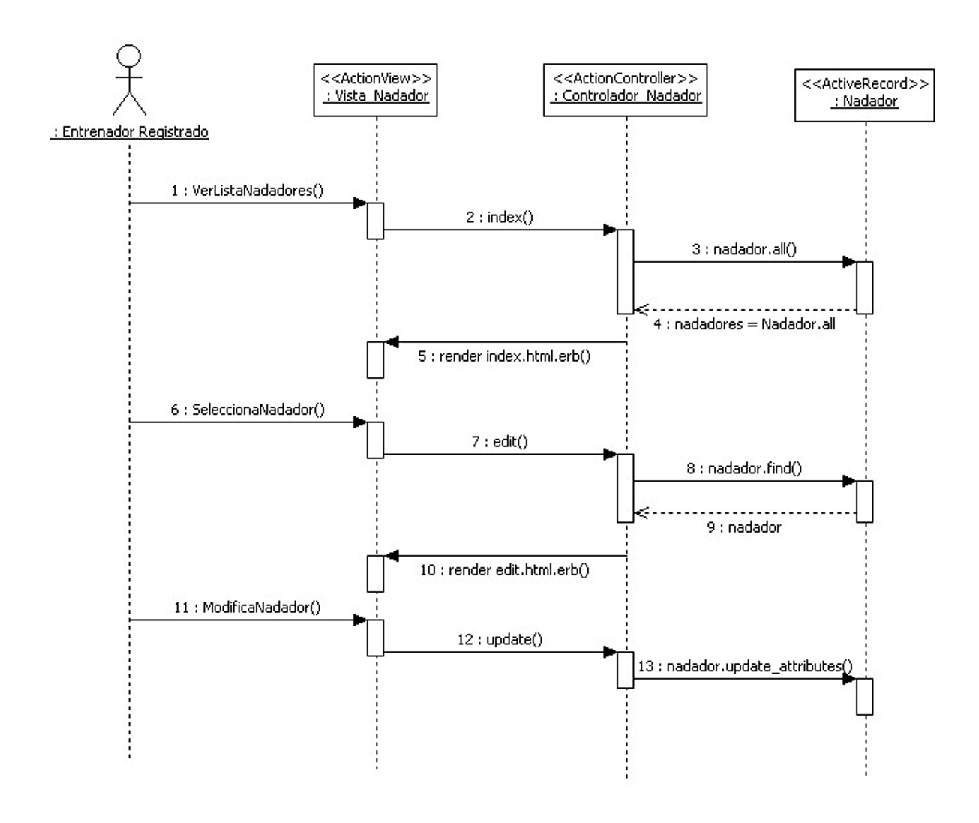
\includegraphics[width=15cm]{./eps/di_diagsecuencia/Nadador_Modificar.eps}
			  \caption{Diagrama de secuencia para modificar un nadador}
			  \label{fig:di_sec_modificarnadador}
			\end{figure}
			
			\newpage
		% subsection diagrama_secuencia_modificar_nadador (end)
		
		% ----------------------------------
		% Sub Diagrama secuencia añadir entrenamiento
		% ----------------------------------
		\subsection{Diagrama secuencia añadir entrenamiento} % (fold)
		  \label{sub:diagrama_secuencia_anadir_entrenamiento}
		  
		  En el diagrama de secuencia de la figura \ref{fig:di_sec_anadirentrenamiento} se muestra el flujo de acciones correspondiente para poder añadir un entrenamiento perteneciente a un entrenador al sistema.
		  
		  El entrenador registrado selecciona la opción de {\it Añadir Entrenamiento} de la {\it Vista Entrenamiento}. Automáticamente, la aplicación enrutará \footnote{El framework rails utiliza un enrutador para guiar el proceso RESTful con cada una de las cabeceras HTTP} el método {\it new} para cargar las vistas con el formulario de un nuevo entrenamiento.
		  
		  El entrenador rellenará el formulario y lo enviará a través del método {\it create}. Será éste el encargado de crear un nuevo entrenamiento en el modelo de {\it Entrenamiento} y, si previamente se han creado ejercicios asociados al mismo, en el de {\it Ejercicios}.
		  
		  \begin{figure}[H]
			  \centering
			    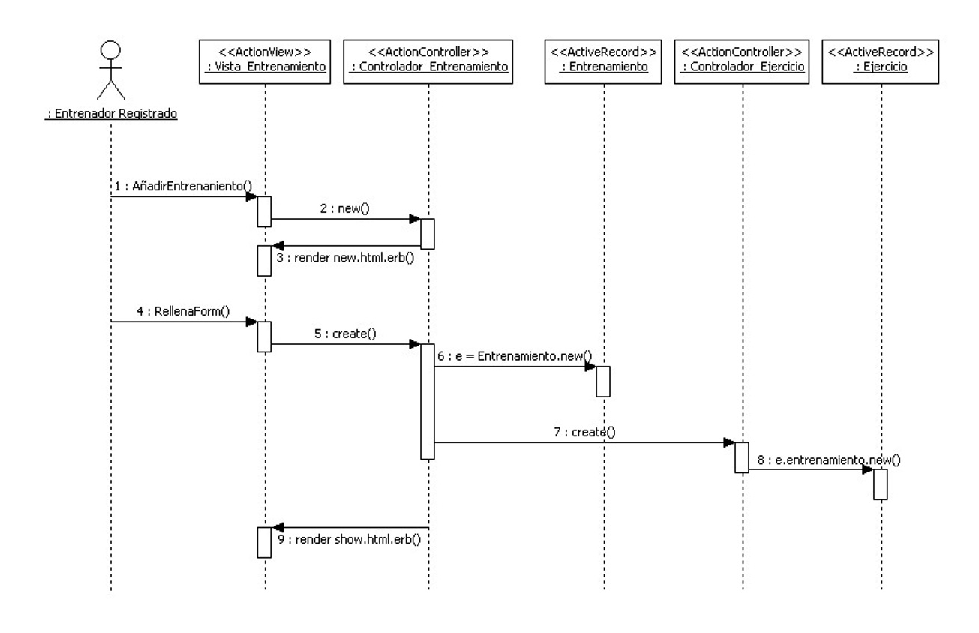
\includegraphics[width=15cm]{./eps/di_diagsecuencia/Entrenamiento_Anadir.eps}
			  \caption{Diagrama de secuencia para añadir un entrenamiento}
			  \label{fig:di_sec_anadirentrenamiento}
			\end{figure}
		
		  \newpage
		% subsection diagrama_secuencia_añadir_entrenamiento (end)
		
		% ----------------------------------
		% Sub Diagrama secuencia ver entrenamiento
		% ----------------------------------
		\subsection{Diagrama secuencia ver entrenamiento} % (fold)
		  \label{sub:diagrama_secuencia_ver_entrenamiento}
		  
		  En el diagrama de secuencia de la figura \ref{fig:di_sec_verentrenamiento} se muestra el flujo de acciones correspondiente para poder ver un entrenamiento perteneciente a un entrenador al sistema.
		  
		  Al igual que en procesos anteriores, para poder ver un entrenamiento previamente se ha seleccionado de una lista. Tras la selección, el controlador busca en el modelo por identificador tanto el entrenamiento como los ejercicios asociados al mismo.
		  
		  Requisitos que se tendrán que contemplar en la fase de implementación:
			
			\begin{itemize}
			 \item No se puede acceder a un entrenamiento perteneciente a otro nadador.
			 \item En caso de no poderse acceder, se mostrará mensaje de error.
			\end{itemize}
			
		  \begin{figure}[H]
			  \centering
			    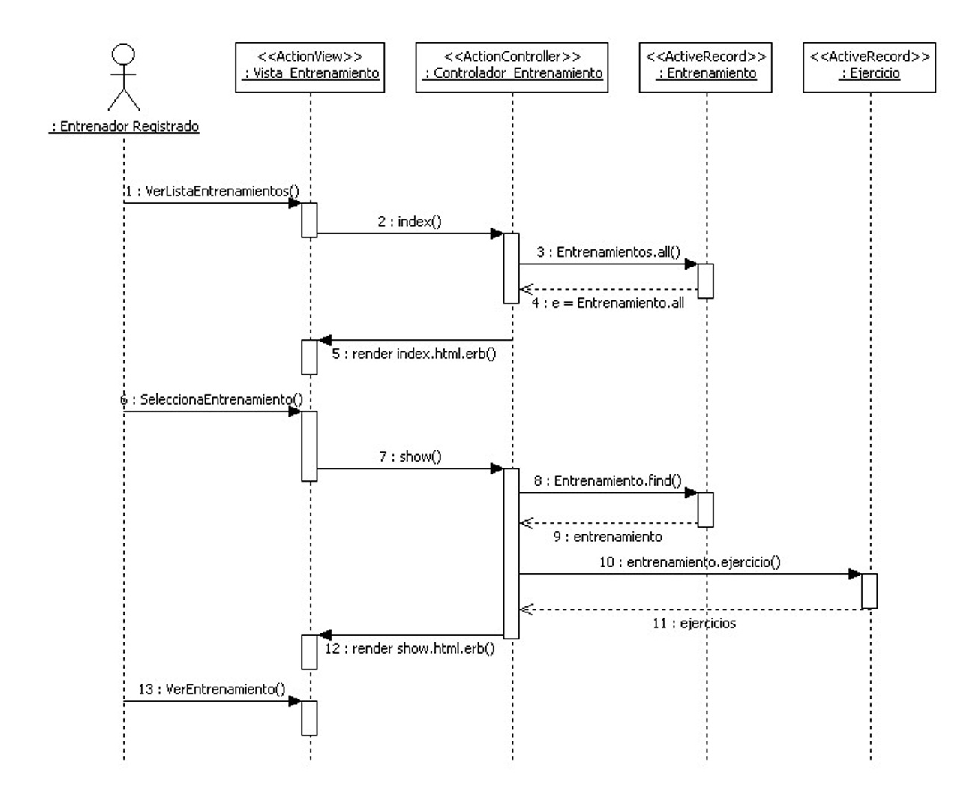
\includegraphics[width=15cm]{./eps/di_diagsecuencia/Entrenamiento_Ver.eps}
			  \caption{Diagrama de secuencia para ver un entrenamiento}
			  \label{fig:di_sec_verentrenamiento}
			\end{figure}
		
		\newpage
		% subsection diagrama_secuencia_ver_entrenamiento (end)
		
		% ----------------------------------
		% Sub Diagrama secuencia para eliminar entrenamiento
		% ----------------------------------
		\subsection{Diagrama secuencia eliminar entrenamiento} % (fold)
		  \label{sub:diagrama_secuencia_eliminar_entrenamiento}
		
		  En el diagrama de secuencia de la figura \ref{fig:di_sec_eliminarentrenamiento} se muestra el flujo de acciones correspondiente para poder eliminar un entrenamiento perteneciente a un entrenador al sistema.
		  
		  Tras seleccionar el entrenamiento a eliminar del listado de entrenamientos totales, la vista hace una llamada al método {\it destroy} del controlador. Éste elimina el registro seleccionado del modelo y posteriormente, los ejercicios asociados al mismo.
		  
		  Aunque para el caso de nadadores (sección \ref{sub:diagrama_secuencia_eliminar_nadador}) no se explicó, surgió la misma analogía que aparecerá en este diagrama. A la hora de borrar los ejercicios, Rails usando el patrón {\it Active Record} (ver sección \ref{ssub:ror_active_record}) genera parte de lo que se conoce como «magia». Internamente el framework implementa un procedimiento para acceder a los ejercicios asociados a un entrenamiento y, a su vez, de habilitar un procedimiento para borrarlos todos.
		  
		  \begin{figure}[H]
			  \centering
			    \includegraphics[width=15cm]{./eps/di_diagsecuencia/Entrenamiento_Eliminar.eps}
			  \caption{Diagrama de secuencia para eliminar un entrenamiento}
			  \label{fig:di_sec_eliminarentrenamiento}
			\end{figure}
		
		  \newpage
		% subsection diagrama_secuencia_para_eliminar_entrenamiento (end)
		
		% ----------------------------------
		% Sub Diagrama secuencia para modificar entrenamiento
		% ----------------------------------
		\subsection{Diagrama secuencia modificar entrenamiento} % (fold)
		  \label{sub:diagrama_secuencia_modificar_entrenamiento}
		  
		  En el diagrama de secuencia de la figura \ref{fig:di_sec_modificarentrenamiento} se muestra el flujo de acciones correspondiente para poder modificar un entrenamiento perteneciente a un entrenador al sistema.
		  
		  \begin{figure}[H]
			  \centering
			    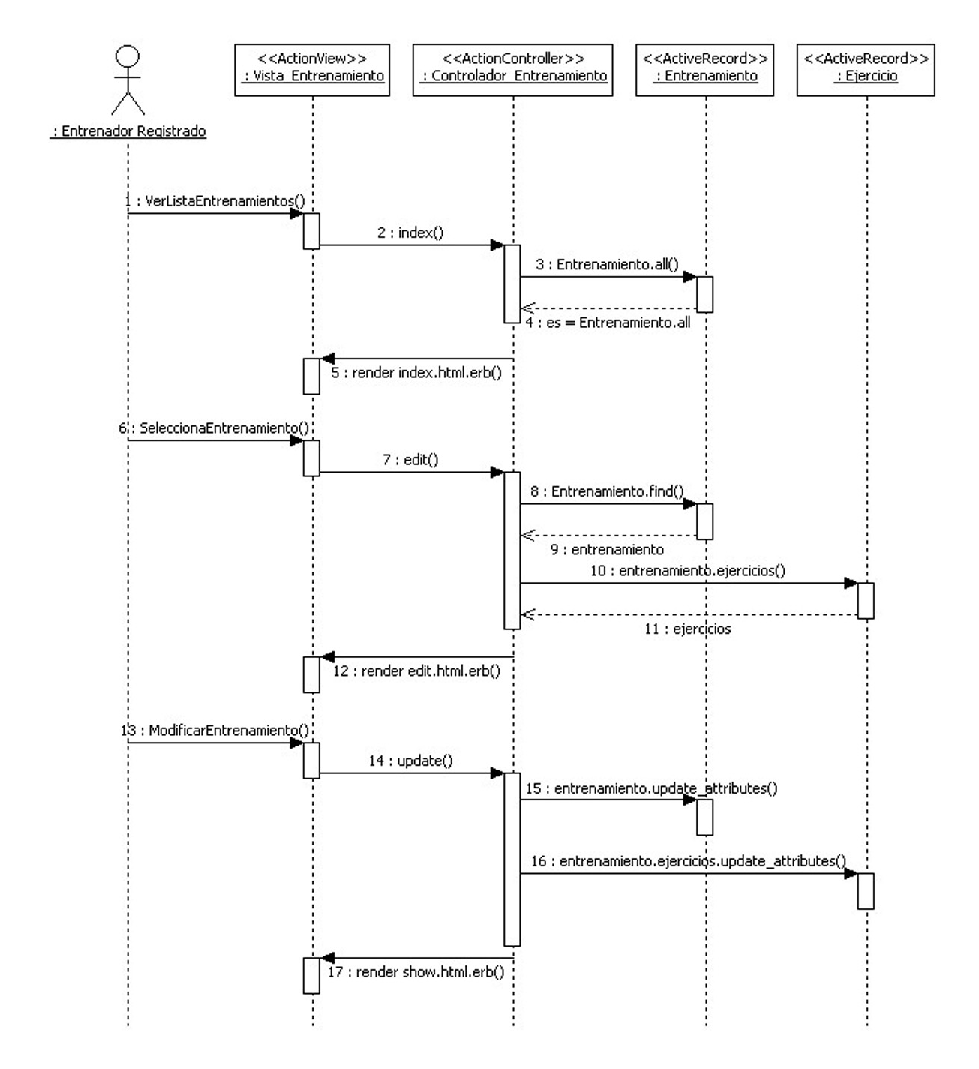
\includegraphics[width=15cm]{./eps/di_diagsecuencia/Entrenamiento_Modificar.eps}
			  \caption{Diagrama de secuencia para modificar un entrenamiento}
			  \label{fig:di_sec_modificarentrenamiento}
			\end{figure}
			
			\newpage
		% subsection diagrama_secuencia_para_modificar_entrenamiento (end)
		
		% ----------------------------------
		% Sub Diagrama secuencia para añadir competición
		% ----------------------------------
		\subsection{Diagrama secuencia añadir competición} % (fold)
		  \label{sub:diagrama_secuencia_anadir_competicion}
		
		  En el diagrama de secuencia de la figura \ref{fig:di_sec_anadircompeticion} se muestra el flujo de acciones correspondiente para poder añadir una competición perteneciente a un entrenador al sistema.
		  
		  \begin{figure}[H]
			  \centering
			    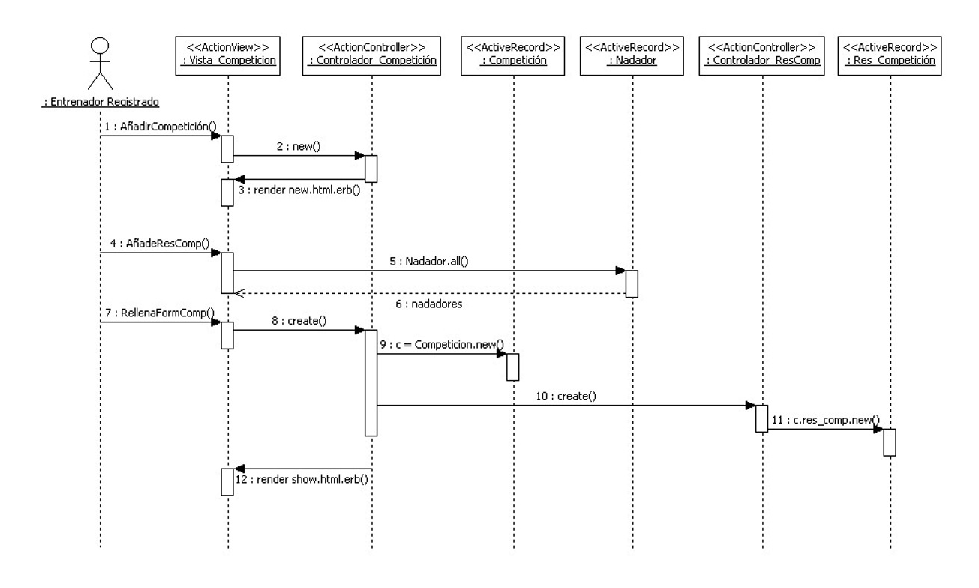
\includegraphics[width=15cm]{./eps/di_diagsecuencia/Competicion_Anadir.eps}
			  \caption{Diagrama de secuencia para añadir una competición}
			  \label{fig:di_sec_anadircompeticion}
			\end{figure}
			
			\newpage
		% subsection diagrama_secuencia_para_añadir_competición (end)
		
		% ----------------------------------
		% Sub Diagrama secuencia para ver competición
		% ----------------------------------
		\subsection{Diagrama secuencia ver competición} % (fold)
		  \label{sub:diagrama_secuencia_ver_competicion}
		  
		  En el diagrama de secuencia de la figura \ref{fig:di_sec_vercompeticion} se muestra el flujo de acciones correspondiente para poder ver una competición perteneciente a un entrenador al sistema.
		  
		  \begin{figure}[H]
			  \centering
			    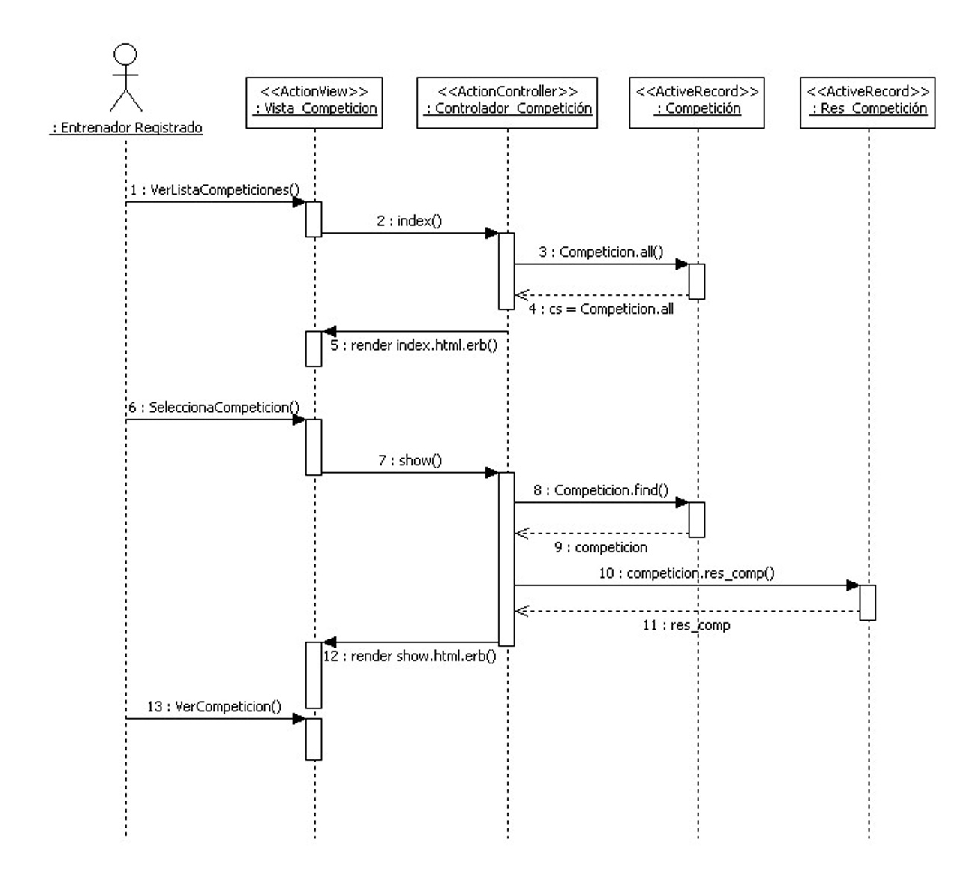
\includegraphics[width=15cm]{./eps/di_diagsecuencia/Competicion_Ver.eps}
			  \caption{Diagrama de secuencia para ver una competición}
			  \label{fig:di_sec_vercompeticion}
			\end{figure}
		
		  \newpage
		% subsection diagrama_secuencia_para_ver_competición (end)
		
		% ----------------------------------
		% Sub Diagrama secuencia para eliminar competición
		% ----------------------------------
		\subsection{Diagrama secuencia eliminar competición} % (fold)
		  \label{sub:diagrama_secuencia_eliminar_competicion}
		  
		  En el diagrama de secuencia de la figura \ref{fig:di_sec_eliminarcompeticion} se muestra el flujo de acciones correspondiente para poder eliminar una competición perteneciente a un entrenador al sistema.
		  
		  \begin{figure}[H]
			  \centering
			    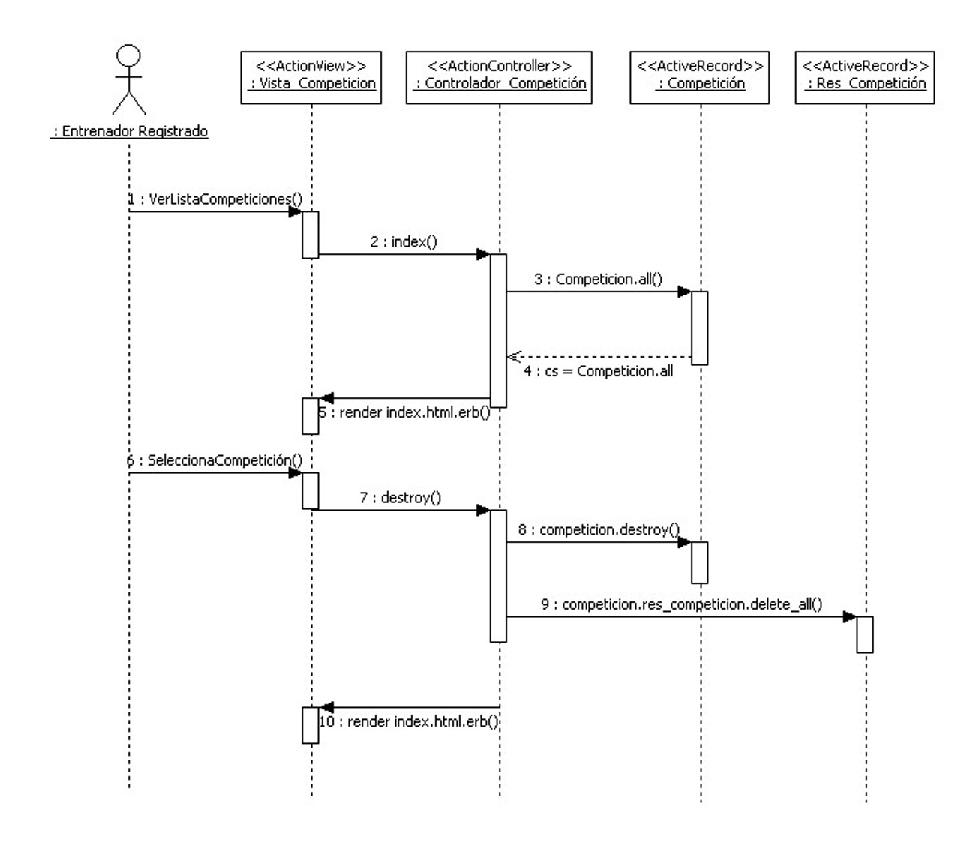
\includegraphics[width=15cm]{./eps/di_diagsecuencia/Competicion_Eliminar.eps}
			  \caption{Diagrama de secuencia para eliminar una competición}
			  \label{fig:di_sec_eliminarcompeticion}
			\end{figure}
		
		  \newpage
		% subsection diagrama_secuencia_para_eliminar_competición (end)
		
		% ----------------------------------
		% Sub Diagrama secuencia para modificar competición
		% ----------------------------------
		\subsection{Diagrama secuencia modificar competición} % (fold)
		  \label{sub:diagrama_secuencia_modificar_competicion}
		  
		  En el diagrama de secuencia de la figura \ref{fig:di_sec_modificarcompeticion} se muestra el flujo de acciones correspondiente para poder modificar una competición perteneciente a un entrenador al sistema.
		  
		  \begin{figure}[H]
			  \centering
			    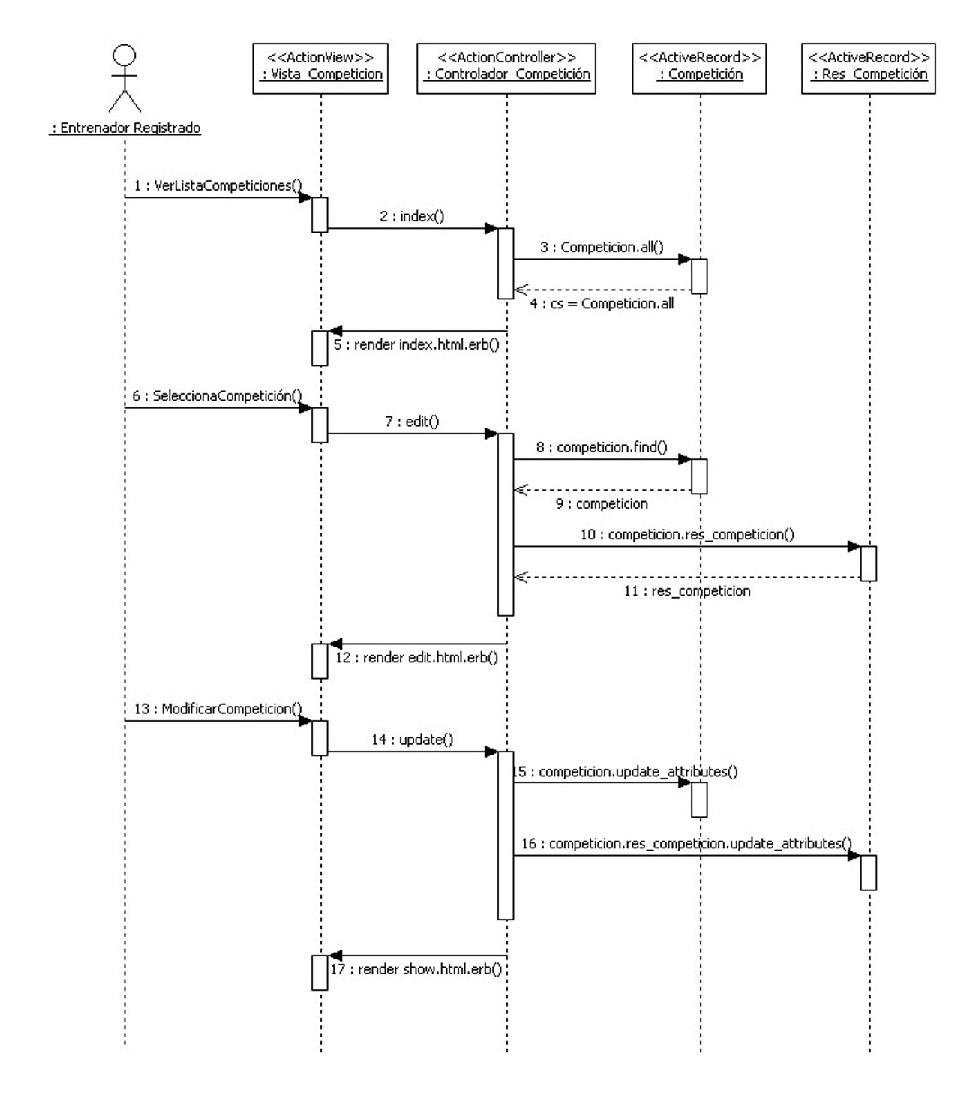
\includegraphics[width=15cm]{./eps/di_diagsecuencia/Competicion_Modificar.eps}
			  \caption{Diagrama de secuencia para modificar una competición}
			  \label{fig:di_sec_modificarcompeticion}
			\end{figure}
		
		  \newpage
		% subsection diagrama_secuencia_para_modificar_competición (end)
		
		% ----------------------------------
		% Sub Diagrama secuencia para añadir test
		% ----------------------------------
		\subsection{Diagrama secuencia añadir test} % (fold)
		  \label{sub:diagrama_secuencia_anadir_test}
		
		  En el diagrama de secuencia de la figura \ref{fig:di_sec_anadirtest} se muestra el flujo de acciones correspondiente para poder añadir un test perteneciente a un entrenador al sistema.
		  
		  \begin{figure}[H]
			  \centering
			    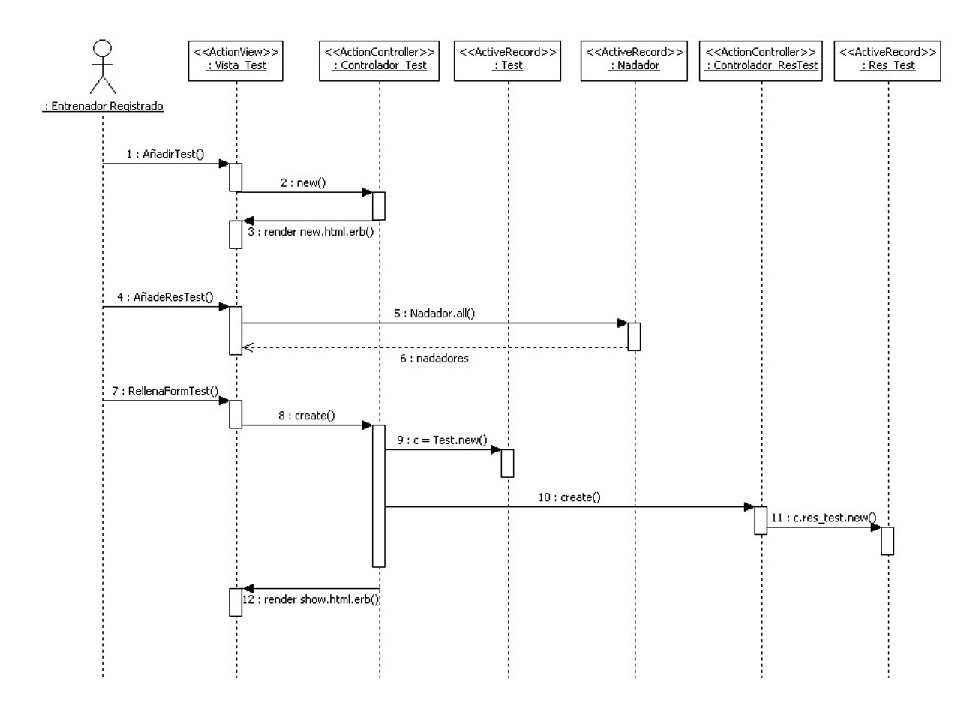
\includegraphics[width=15cm]{./eps/di_diagsecuencia/Test_Anadir.eps}
			  \caption{Diagrama de secuencia para añadir un test}
			  \label{fig:di_sec_anadirtest}
			\end{figure}
			
			\newpage
		% subsection diagrama_secuencia_para_añadir_test (end)
		
		% ----------------------------------
		% Sub Diagrama secuencia para ver test
		% ----------------------------------
		\subsection{Diagrama secuencia ver test} % (fold)
		  \label{sub:diagrama_secuencia_ver_test}
		  
		  En el diagrama de secuencia de la figura \ref{fig:di_sec_vertest} se muestra el flujo de acciones correspondiente para poder ver un test perteneciente a un entrenador al sistema.
		  
		  \begin{figure}[H]
			  \centering
			    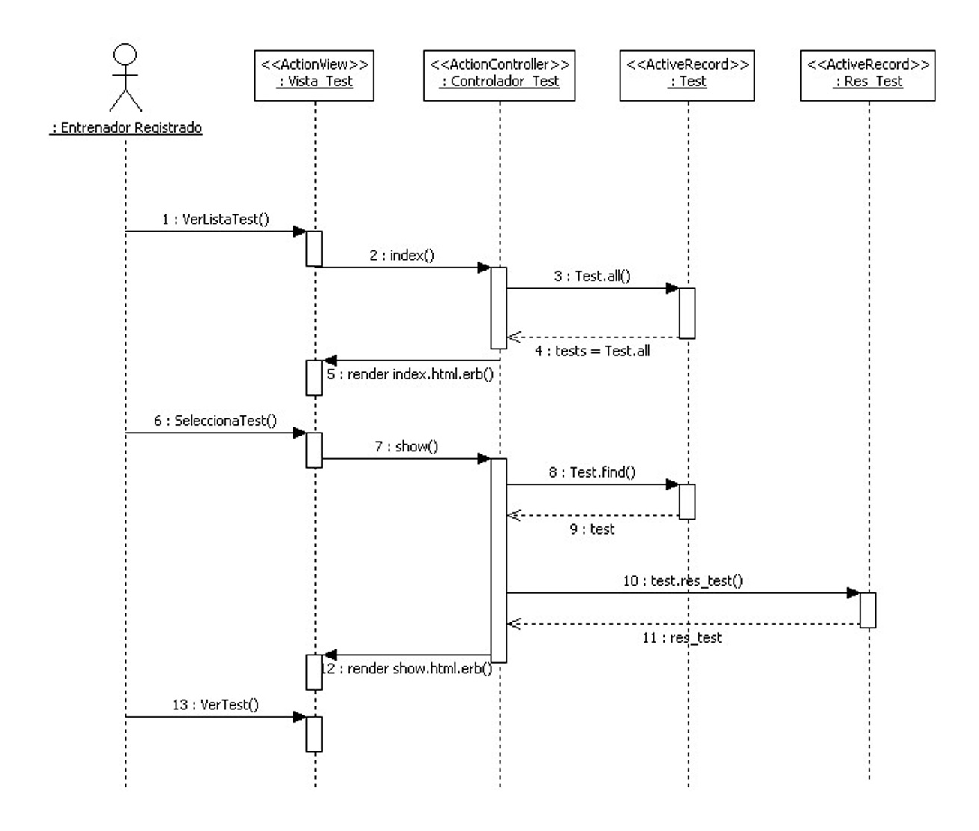
\includegraphics[width=15cm]{./eps/di_diagsecuencia/Test_Ver.eps}
			  \caption{Diagrama de secuencia para ver un test}
			  \label{fig:di_sec_vertest}
			\end{figure}
		
		  \newpage
		% subsection diagrama_secuencia_para_ver_test (end)
		
		% ----------------------------------
		% Sub Diagrama secuencia para eliminar test
		% ----------------------------------
		\subsection{Diagrama secuencia eliminar test} % (fold)
		  \label{sub:diagrama_secuencia_eliminar_test}
		
		  En el diagrama de secuencia de la figura \ref{fig:di_sec_eliminartest} se muestra el flujo de acciones correspondiente para poder añadir un eliminar perteneciente a un entrenador al sistema.
		  
		  \begin{figure}[H]
			  \centering
			    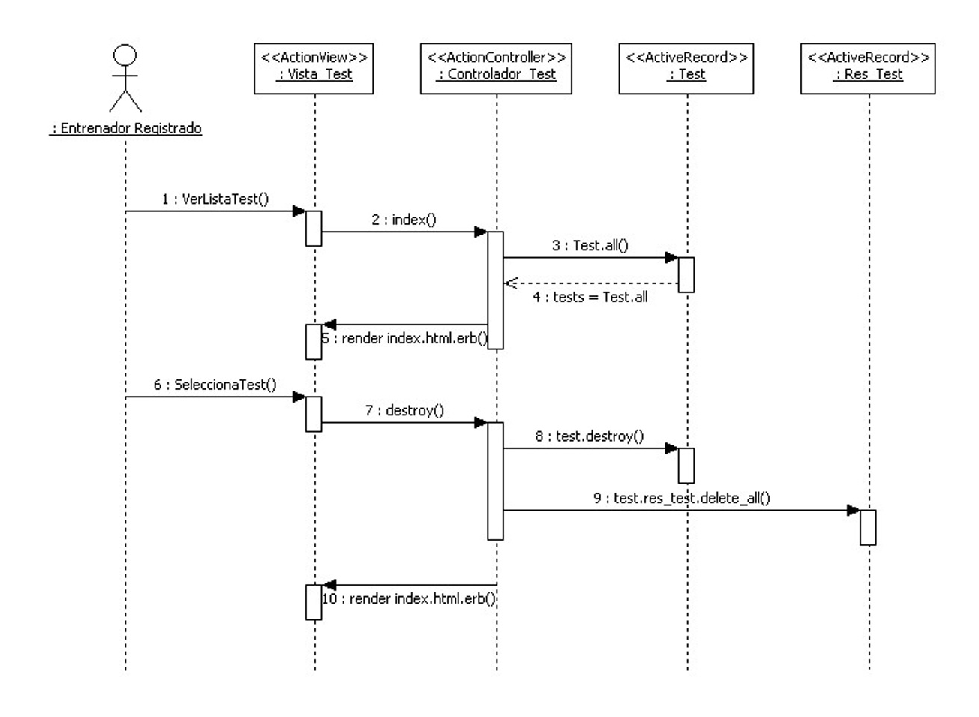
\includegraphics[width=15cm]{./eps/di_diagsecuencia/Test_Eliminar.eps}
			  \caption{Diagrama de secuencia para eliminar un test}
			  \label{fig:di_sec_eliminartest}
			\end{figure}
			
			\newpage
		% subsection diagrama_secuencia_para_eliminar_test (end)
		
		% ----------------------------------
		% Sub Diagrama secuencia para modificar test
		% ----------------------------------
		\subsection{Diagrama secuencia modificar test} % (fold)
		  \label{sub:diagrama_secuencia_modificar_test}
		
		  En el diagrama de secuencia de la figura \ref{fig:di_sec_modificartest} se muestra el flujo de acciones correspondiente para poder modificar un test perteneciente a un entrenador al sistema.
		  
		  \begin{figure}[H]
			  \centering
			    \includegraphics[width=15cm]{./eps/di_diagsecuencia/Test_Modificar.eps}
			  \caption{Diagrama de secuencia para modificar un test}
			  \label{fig:di_sec_modificartest}
			\end{figure}
			
			\newpage
		% subsection diagrama_secuencia_para_modificar_test (end)
		
		% ----------------------------------
		% Sub Diagrama secuencia añadir incidencia
		% ----------------------------------
		\subsection{Diagrama secuencia añadir incidencia} % (fold)
		  \label{sub:diagrama_secuencia_anadir_incidencia}
		
		  En el diagrama de secuencia de la figura \ref{fig:di_sec_anadirincidencia} se muestra el flujo de acciones correspondiente para poder añadir una incidencia perteneciente a un entrenador al sistema.
		  
		  \begin{figure}[H]
			  \centering
			    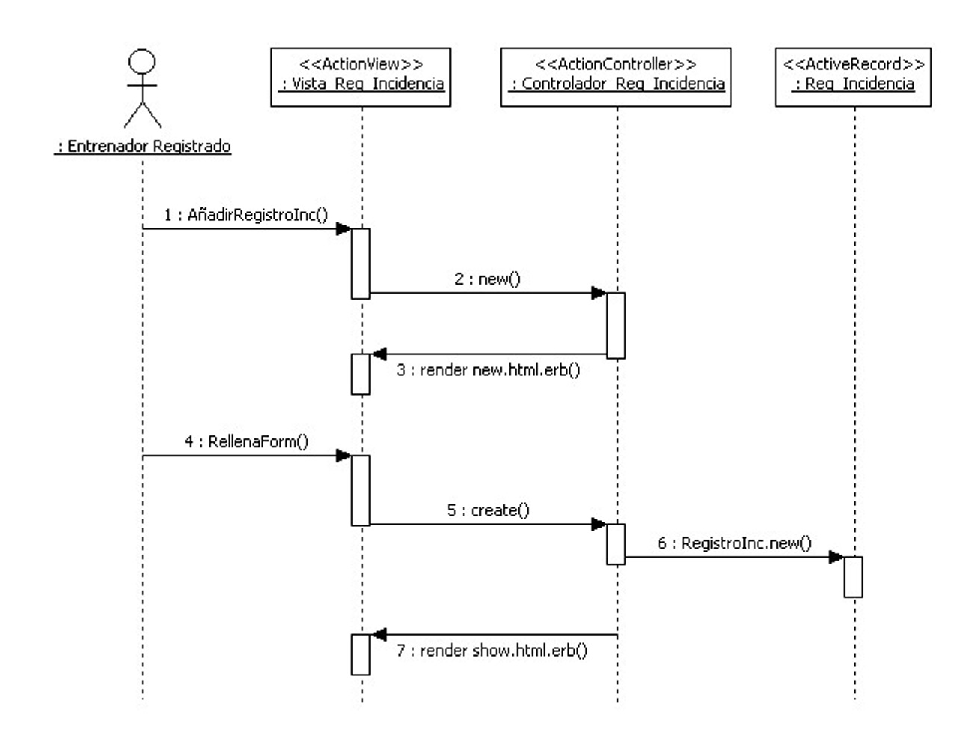
\includegraphics[width=15cm]{./eps/di_diagsecuencia/RegistroInc_Anadir.eps}
			  \caption{Diagrama de secuencia para modificar una incidencia}
			  \label{fig:di_sec_anadirincidencia}
			\end{figure}
			
			\newpage
		% subsection diagrama_secuencia_añadir_incidencia (end)
		
		% ----------------------------------
		% Sub Diagrama secuencia ver incidencia
		% ----------------------------------
		\subsection{Diagrama secuencia ver incidencia} % (fold)
		  \label{sub:diagrama_secuencia_ver_incidencia}
		
		  En el diagrama de secuencia de la figura \ref{fig:di_sec_verincidencia} se muestra el flujo de acciones correspondiente para poder ver una incidencia perteneciente a un entrenador al sistema.
		  
		  \begin{figure}[H]
			  \centering
			    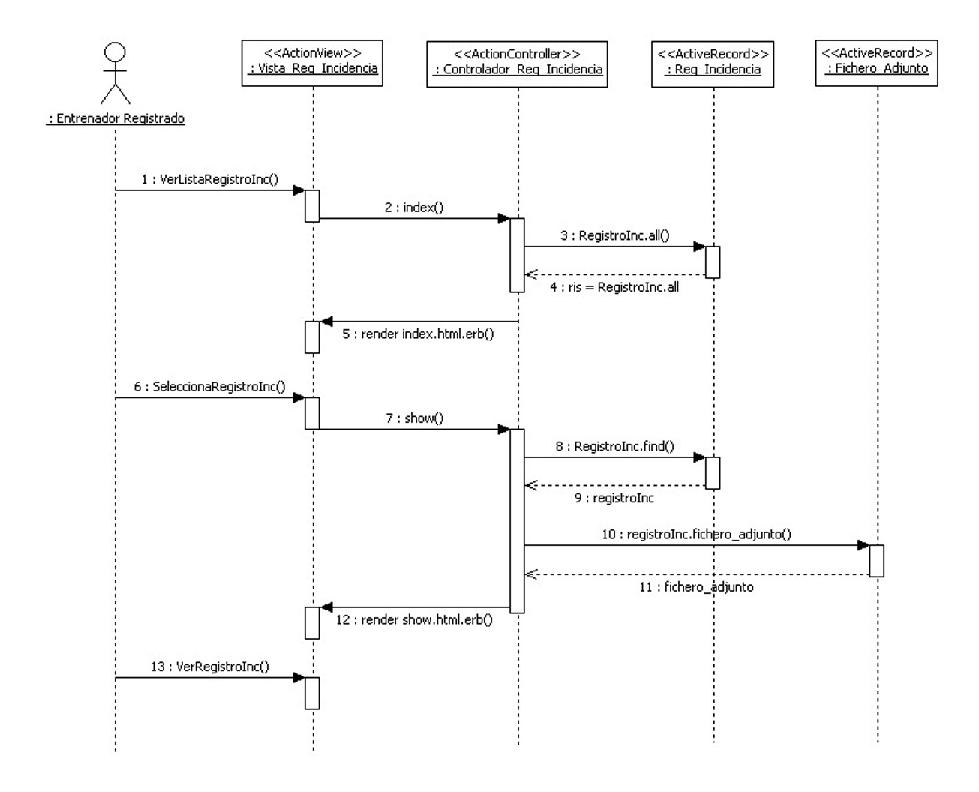
\includegraphics[width=15cm]{./eps/di_diagsecuencia/RegistroInc_Ver.eps}
			  \caption{Diagrama de secuencia para ver una incidencia}
			  \label{fig:di_sec_verincidencia}
			\end{figure}
			
			\newpage
		% subsection diagrama_secuencia_ver_incidencia (end)
		
		% ----------------------------------
		% Sub Diagrama secuencia eliminar incidencia
		% ----------------------------------
		\subsection{Diagrama secuencia eliminar incidencia} % (fold)
		  \label{sub:diagrama_secuencia_eliminar_incidencia}
		
		  En el diagrama de secuencia de la figura \ref{fig:di_sec_eliminarincidencia} se muestra el flujo de acciones correspondiente para poder eliminar una incidencia perteneciente a un entrenador al sistema.
		  
		  \begin{figure}[H]
			  \centering
			    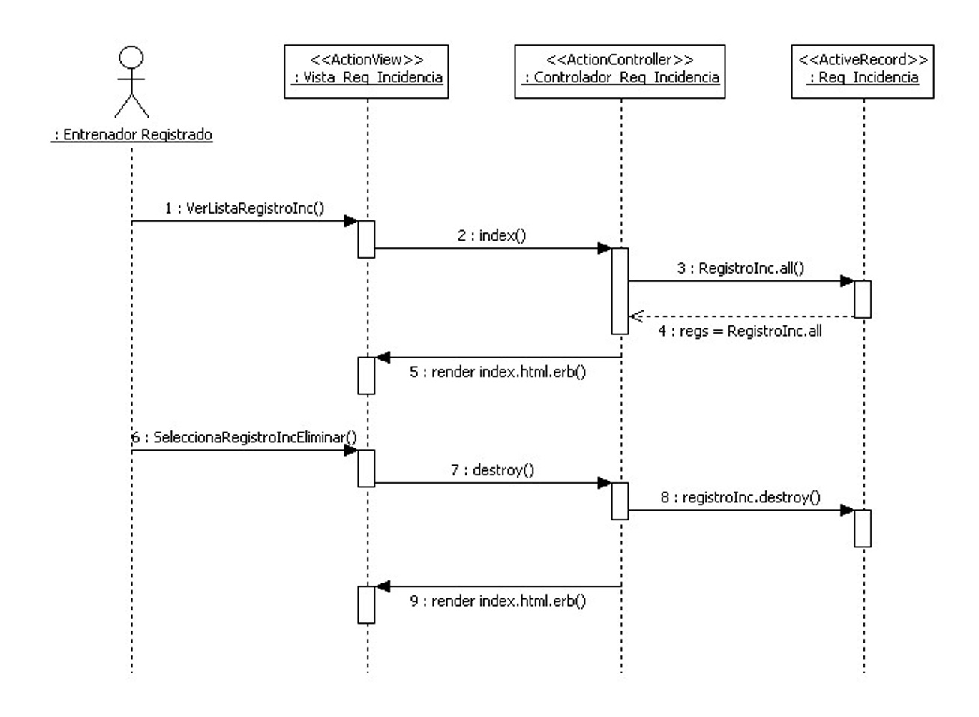
\includegraphics[width=15cm]{./eps/di_diagsecuencia/RegistroInc_Eliminar.eps}
			  \caption{Diagrama de secuencia para eliminar una incidencia}
			  \label{fig:di_sec_eliminarincidencia}
			\end{figure}
			
			\newpage
		% subsection diagrama_secuencia_eliminar_incidencia (end)
		
		% ----------------------------------
		% Sub Diagrama secuencia modificar incidencia
		% ----------------------------------
		\subsection{Diagrama secuencia modificar incidencia} % (fold)
		  \label{sub:diagrama_secuencia_modificar_incidencia}
		
		  En el diagrama de secuencia de la figura \ref{fig:di_sec_modificarincidencia} se muestra el flujo de acciones correspondiente para poder modificar una incidencia perteneciente a un entrenador al sistema.
		  
		  \begin{figure}[H]
			  \centering
			    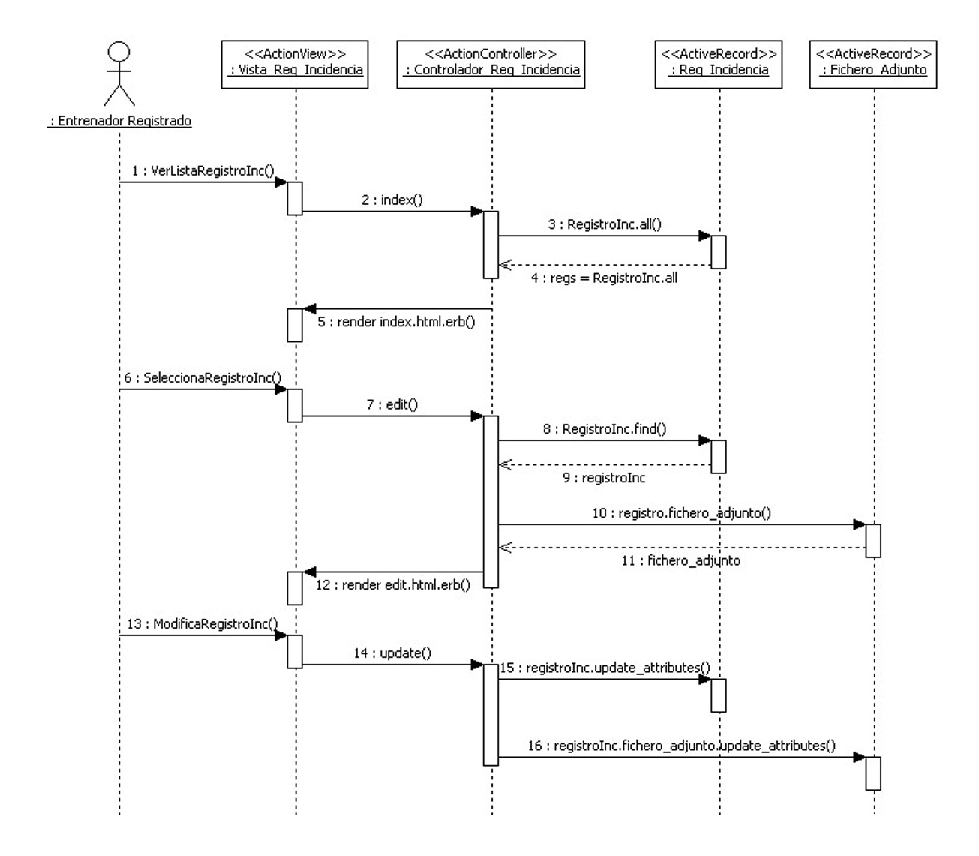
\includegraphics[width=15cm]{./eps/di_diagsecuencia/RegistroInc_Modificar.eps}
			  \caption{Diagrama de secuencia para modificar una incidencia}
			  \label{fig:di_sec_modificarincidencia}
			\end{figure}
			
		% subsection diagrama_secuencia_modificar_incidencia (end)
	% section diagramas_de_secuencia (end)

	% ----------------------------------
	% Sec Diagrama de paquetes
	% ----------------------------------
	\section{Diagrama de paquetes} % (fold)
		\label{sec:diagrama_de_paquetes_diseno}
	
		En la sección \ref{sec:diagrama_de_paquetes_analisis} de la fase de análisis se hace una primera aproximación de las capas necesarias de la aplicación. Se hizo referencia a una arquitectura en 4 capas donde se detalló la composición de las capas genérica y específica. El siguiente paso es identificar los subsistemas intermedios y de software del sistema.
		
		El software del sistema y la capa intermedia constituyen los cimientos de un sistema, ya que toda la funcionalidad descansa sobre software como sistemas operativos, sistemas de gestión de bases de datos, software de comunicaciones, tecnologías de distribución de objetos, kits de diseño de IGU y tecnologías de gestión de transacciones. La selección e integración de productos software que se comprar o se construyen son dos de los objetivos fundamentales durante las fases de inicio y elaboración de un proyecto. En una organización, son los arquitectos quienes verifican que los productos software elegidos encajan en la arquitectura y permiten una implementación económica del sistema. 
		
		Debido a que se usará el {\it framework rails}, la capa intermedia se compondrá básicamente por las gemas (equivalente a componentes) ruby que se necesitarán. Tanto las capas específicas como genéricas dependerán de ellas para una integración total del sistema. Además, por el tipo de aplicación, la cuarta capa ---software del sistema--- se encuentra vacía.
		
		\begin{figure}[H]
		  \centering
		    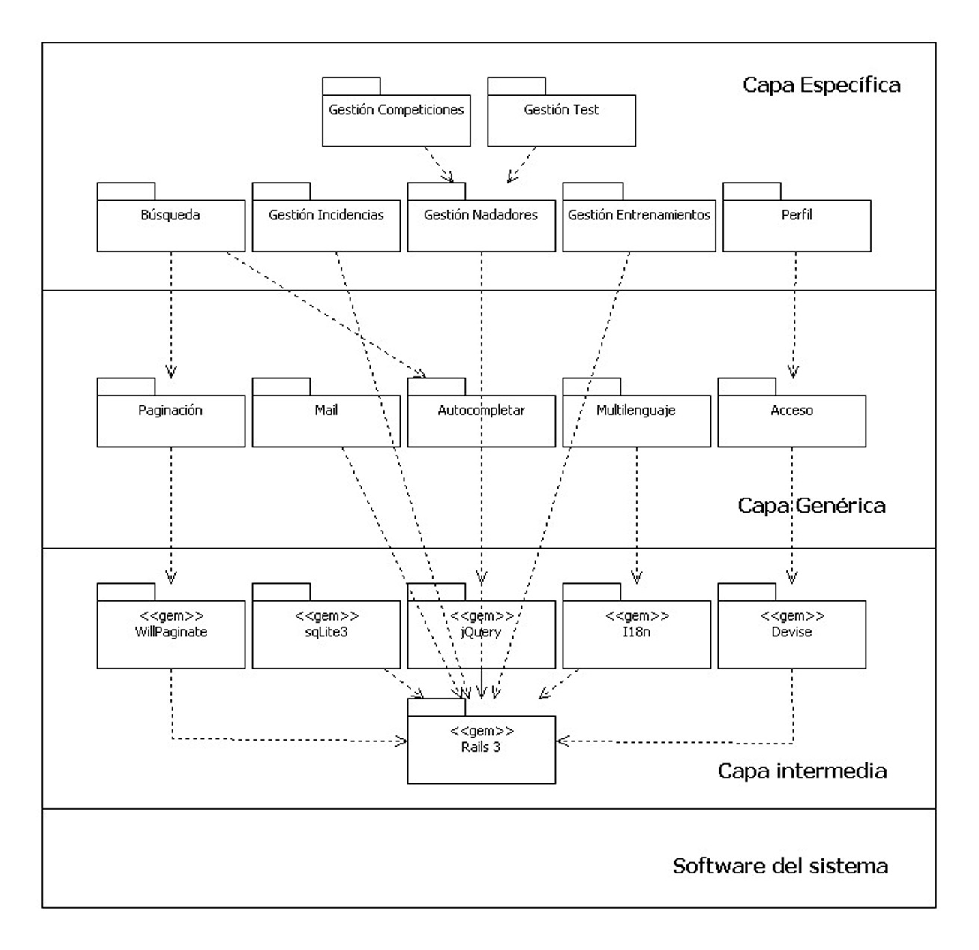
\includegraphics[width=16cm]{./eps/di_diagpaquetes/di_diagpaquetes.eps}
		  \caption{Diagrama de paquetes con subsistemas de las capas intermedia y de software del sistema}
		  \label{fig:di_sec_vernadador}
		\end{figure}
		
		Para poder integrar los subsistemas de la capa específica, el {\it framework} cuenta con el soporte de clases internas que dan forma al patrón MVC. Éstas serán las que aparecen como estereotipos en el diagrama de clases que aparece en la figura \ref{fig:di_diag_clases}. 
	
	% section diagrama_de_paquetes (end)

	% ----------------------------------
	% Sec Modelo de despliegue
	% ----------------------------------
	\section{Modelo de despliegue} % (fold)
		\label{sec:modelo_de_despliegue}
	
		El modelo de despliegue es un modelo de objetos que describe la distribución física del sistema en términos de cómo se distribuye la funcionalidad entre los nodos de cómputo. El modelo de despliegue se utiliza como entrada fundamental en las actividades de diseño e implementación debido a que la distribución tiene una influencia principal en su diseño.
		
		Se puede observar lo siguiente sobre el modelo de despliegue:
		\begin{itemize}
			\item Cada nodo representa un recurso de cómputo, normalmente un procesador o un dispositivo hardware similar.
			\item Los nodos poseen relaciones que representan medios de comunicación entre ellos, tales como {\it internet, intranet, bus y similares}.
			\item El modelo de despliegue puede describir diferentes configuraciones de red, incluidas las configuraciones para pruebas y para simulación.
			\item La funcionalidad (los procesos) de un nodo se definen por los componentes que se distribuyen sobre ese nodo.
			\item El modelo de despliegue en sí mismo representa una correspondencia entre la arquitectura {\it software} y la arquitectura {\it del sistema} (hardware).
		\end{itemize}
	
		\begin{figure}[H]
		  \centering
		    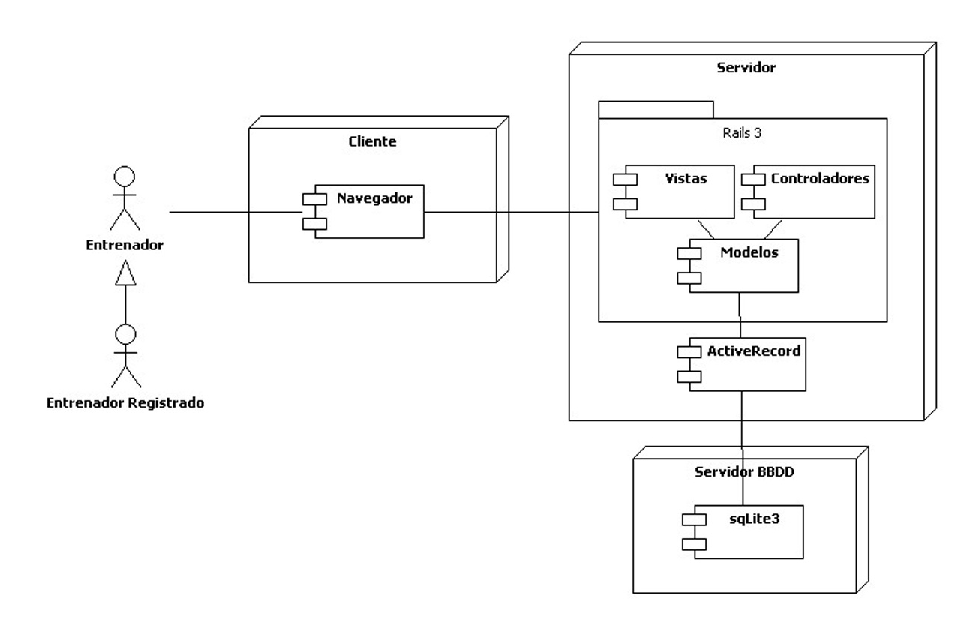
\includegraphics[width=14cm]{./eps/di_diagdespliegue/di_diagdespliegue.eps}
		  \caption{Diagrama de despliegue}
		  \label{fig:di_diag_despliegue}
		\end{figure}
		
		La figura \ref{fig:di_diag_despliegue} hace referencia al diagrama de despliegue de la aplicación. El actor principal actúa en el {\bf nodo cliente} a través del navegador. Desde él se conecta usando la red de internet mediante protocolo http/https con el {\bf nodo servidor}. 
		
		En el nodo servidor se encuentran los subsistemas definidos desde la fase de análisis. En el diagrama, por simplificación, se muestran cada uno de los componentes que representan el patrón MVC, obviando que cada uno de ellos incluye los paquetes de la capa específica y genérica del sistema. La gema {\it ActiveRecord} actúa de interfaz con el SGBD.
		
	% section modelo_de_despliegue (end)
	
% chapter diseño (end)